\documentclass[11pt,twoside,titlepage,a4paper]{article}

%%%%%%%%%%%%%%%%%%%%%%%%%%%%%%%%%%%%%%%%%%%%%%%%%%%%%%%%%%%%%%%%%%%%%%%%%%%%%%%
% PAQUETES
%salu2 - Valentino
\usepackage{xcolor} % Colores
\usepackage[xcolor]{mdframed} % Marcos
\usepackage{amsmath} % Matemáticas
\usepackage{amsfonts} % Letras caligráficas para matemáticas
\usepackage{mathtools} % Matemáticas extra
\usepackage{amsthm} % Teoremas
\usepackage{listingsutf8} % Código
\usepackage[a4paper]{geometry} % Márgenes
\usepackage{enumitem} % Opciones de personalización de listas
\usepackage{fancyhdr} % Encabezado / Pie de página
\usepackage{titlesec} % Títulos
\usepackage{pagecolor} % Colorear las portadas
\usepackage{graphicx} % Imágenes
\usepackage{hyperref} % Referencias
\usepackage{sidenotes} % Notas en el margen
\usepackage{pgfplots} % Gráficos de funciones
\usepackage{biblatex} % Bibliografía
\bibliography{bibliografia.bib}
\usepackage{caption}
\usepackage{subcaption}
%%%%%%%%%%%%%%%%%%%%%%%%%%%%%%%%%%%%%%%%%%%%%%%%%%%%%%%%%%%%%%%%%%%%%%%%%%%%%%%
% COMANDOS PERSONALIZADOS

% Año o cualquier otra información para la portada
\newcommand{\fecha}{
\today
}
% Autores del documento
\newcommand{\autores}{
Exequiel Alberto Castro Rivero y Blanca Cano Camarero
}

\newcommand{\margenimagen}{
\newgeometry{
    left=2.5cm, % Margen izquierdo
	right=5cm, % Margen derecho
	bottom=2.5cm % Margen inferior}
}
}

%%%%%%%%%%%%%%%%%%%%%%%%%%%%%%%%%%%%%%%%%%%%%%%%%%%%%%%%%%%%%%%%%%%%%%%%%%%%%%%
% TIPOGRAFÍA

\usepackage{heuristica}
\usepackage[heuristica,vvarbb,bigdelims]{newtxmath}
\usepackage[T1]{fontenc}
\renewcommand*\oldstylenums[1]{\textosf{#1}}
\usepackage[spanish]{babel}

%%%%%%%%%%%%%%%%%%%%%%%%%%%%%%%%%%%%%%%%%%%%%%%%%%%%%%%%%%%%%%%%%%%%%%%%%%%%%%%
% DEFINICIÓN DE COLORES

% COLORES DE LA ESTRUCTURA DEL DOCUMENTO
\definecolor{bg_por}{HTML}{8A0808} % Portada
\definecolor{fg_por}{HTML}{FFFFFF} % Texto de la portada
\definecolor{fg_sec}{HTML}{8A0808} % Títulos de las secciones
\definecolor{fg_ssec}{HTML}{610505} % Títulos de las subsecciones
\definecolor{fg_sssec}{HTML}{300303} % Títulos de las subsubsecciones
\definecolor{fg_head}{HTML}{610B0B} % Texto del encabezado
% COLORES PARA CÓDIGO
\definecolor{li_code}{HTML}{8A0808} % Línea a la izquierda
\definecolor{rw_code}{HTML}{610B0B} % Palabras reservadas
\definecolor{st_code}{HTML}{300303} % Cadenas de caracteres
\definecolor{cm_code}{HTML}{333333} % Comentarios
% COLORES PARA LISTAS
\definecolor{l_1}{HTML}{8A0808} % Primer símbolo
\definecolor{l_2}{HTML}{610505} % Primera indentación
\definecolor{l_3}{HTML}{300303} % Segunda indentación
\definecolor{l_4}{HTML}{000000} % Tercera indentación
% COLORES PARA MARCOS
\definecolor{li_ejs}{HTML}{8A0808} % Línea marco ejemplos
\definecolor{li_defs}{HTML}{610505} % Línea marco definiciones
\definecolor{bg_ejs}{HTML}{FFEDEE} % Fondo ejemplos
\definecolor{bg_defs}{HTML}{FFE0DF} % Fondo definiciones
% COLORES PARA REFERENCIAS
\definecolor{fg_url}{HTML}{610505} % Links


%%%%%%%%%%%%%%%%%%%%%%%%%%%%%%%%%%%%%%%%%%%%%%%%%%%%%%%%%%%%%%%%%%%%%%%%%%%%%%%
% REFERENCIAS

\hypersetup{
	pdftitle={	Implementación de las técnicas de mezcla de regiones usando la ecuación de Poisson}, % Título del pdf
	pdfauthor={}, % Autor del pdf
    colorlinks=true, % Referencias con color
    linkcolor=black, % Color de las referencias internas
    urlcolor=fg_url, % Color de los links
    citecolor=fg_ssec, % Color de las referencias
}
\urlstyle{same} % Links con el mismo tipo de letra

%%%%%%%%%%%%%%%%%%%%%%%%%%%%%%%%%%%%%%%%%%%%%%%%%%%%%%%%%%%%%%%%%%%%%%%%%%%%%%%
% TEOREMAS

\numberwithin{equation}{section} % Numeración de ecuaciones
% Teoremas-Lemas-Definiciones-Corolarios
\newtheoremstyle{usual} % Nombre del estilo
{} % Espacio por encima
{} % Espacio por debajo
{} % Estilo del cuerpo
{} % Indentación
{\bfseries} % Estilo de la cabecera
{} % Símbolo tras la cabecera
{ } % Espacio tras la cabecera
{\thmname{#1}\thmnumber{ #2 }\thmnote{(\textit{#3})}:} % Especificación de la cabecera
\theoremstyle{usual}
\newtheorem{theorem}{Teorema}[section] % Comando para los teoremas

%%%%%%%%%%%%%%%%%%%%%%%%%%%%%%%%%%%%%%%%%%%%%%%%%%%%%%%%%%%%%%%%%%%%%%%%%%%%%%%
% CÓDIGO

\lstset{
	basicstyle=\footnotesize\ttfamily, % Estilo del código
	inputencoding=utf8/latin1, % Codificación
	xleftmargin=1.3em, % Margen extra a la izquierda
	breaklines=true, % Romper líneas largas
	language=, % Lenguaje del código
	numbers=left, % Números de línea
	numbersep=8pt, % Separación de los números de línea
	tabsize=4, % Tamaño de los tabs
	frame=leftline, % Posición del enmarcado
	framerule=1pt, % Grosor del enmarcado
	showstringspaces=false, % Mostrar los espacios en las cadenas de caracteres
	keywordstyle=\color{rw_code}, % Estilo de las palabras reservadas
	numberstyle=\normalfont, % Estilo de los números de línea
	rulecolor=\color{li_code}, % Estilo del enmarcado
	commentstyle=\color{cm_code}, % Estilo de los comentarios
	stringstyle=\color{st_code} % Estilo de las cadenas de caracteres
}

%%%%%%%%%%%%%%%%%%%%%%%%%%%%%%%%%%%%%%%%%%%%%%%%%%%%%%%%%%%%%%%%%%%%%%%%%%%%%%%
% MÁRGENES

\geometry{
	left=2.5cm, % Margen izquierdo
	right=2.5cm, % Margen derecho
	bottom=2.5cm % Margen inferior
}

%%%%%%%%%%%%%%%%%%%%%%%%%%%%%%%%%%%%%%%%%%%%%%%%%%%%%%%%%%%%%%%%%%%%%%%%%%%%%%%
% LISTAS/TABLAS

\renewcommand{\arraystretch}{1.3} % Tamaño entre líneas de una tabla
% SÍMBOLOS LISTAS
\renewcommand{\labelitemi}{\color{l_1}$\bullet$} % Primer símbolo
\renewcommand{\labelitemii}{\color{l_2}$\circ$} % Símbolo primera indentación
\renewcommand{\labelitemiii}{\color{l_3}$\diamond$} % Símbolo segunda indentación
\renewcommand{\labelitemiv}{\color{l_4}$-$} % Símbolo tercera indentación
% SÍMBOLOS ENUMERACIONES
\renewcommand{\labelenumi}{\color{l_1}\bfseries\arabic{enumi}.} % Primer símbolo
\renewcommand{\labelenumii}{\color{l_2}\bfseries\Roman{enumii}.} % Símbolo primera indentación
\renewcommand{\labelenumiii}{\color{l_3}\bfseries(\alph{enumiii})} % Símbolo segunda indentación
\renewcommand{\labelenumiv}{\color{l_4}\bfseries\Alph{enumiv}.} % Símbolo tercera indentación
% DESCRIPCIONES
\renewcommand{\descriptionlabel}[1]{\hspace{\labelsep}\color{l_1}\textbf{#1}} % Color y estilo del título de la descripción

%%%%%%%%%%%%%%%%%%%%%%%%%%%%%%%%%%%%%%%%%%%%%%%%%%%%%%%%%%%%%%%%%%%%%%%%%%%%%%%
% ENCABEZADO/PIE DE PAGINA

\setlength{\headheight}{14pt} % Tamaño del encabezado
\pagestyle{fancy}
\fancyhf{}
% Para que aparezca el título de la sección y no el número 
\renewcommand{\sectionmark}[1]{%
\markboth{#1}{}}
% Encabezado
\fancyhead[LE,RO]{\color{fg_head}{\leftmark}} % A la izquierda en pares, derecha en impares
\fancyhead[RE,LO]{\color{fg_head}{}} % A la derecha en pares, izquierda en impares
% Pie de página
\fancyfoot[LE,RO]{\Large\textbf{\thepage}} % A la izquierda en pares, derecha en impares
\renewcommand{\headrulewidth}{0.5pt} % Grosor de la línea

%%%%%%%%%%%%%%%%%%%%%%%%%%%%%%%%%%%%%%%%%%%%%%%%%%%%%%%%%%%%%%%%%%%%%%%%%%%%%%%
% TÍTULOS

% Estilo de las secciones
\titleformat{\section}
{\color{fg_sec}\Huge\bfseries}
{\color{fg_sec}\thesection}{1em}{}
% Estilo de las subsecciones
\titleformat{\subsection}
{\color{fg_ssec}\huge\bfseries}
{\color{fg_ssec}\thesubsection}{1em}{}
% Estilo de las subsecciones
\titleformat{\subsubsection}
{\color{fg_sssec}\LARGE\bfseries}
{\color{fg_sssec}\thesubsubsection}{1em}{}

%%%%%%%%%%%%%%%%%%%%%%%%%%%%%%%%%%%%%%%%%%%%%%%%%%%%%%%%%%%%%%%%%%%%%%%%%%%%%%%
% MISCELÁNEO

\renewcommand{\contentsname}{Índice} % Cambiar el título del índice
\setlength\parindent{0pt} % Tamaño de la sangría


\begin{document}
%%%%%%%%%%%%%%%%%%%%%%%%%%%%%%%%%%%%%%%%%%%%%%%%%%%%%%%%%%%%%%%%%%%%%%%%%%%%%%%
% PORTADA

\begin{titlepage}
	\newpagecolor{bg_por} % Color de la portada
	\centering
	
\includegraphics[width=0.7\textwidth]{imagenes/ugr_logo.jpg} \\ % Logo
	\vspace{7em}
	\centering
	\color{fg_por}{
	%\title{Implementación de la técnica de mezclado de colores usando la ecuación del Poisson}
		\fontsize{50pt}{50pt}{\scshape{
		Implementación\\
		de técnicas \\
		de mezcla de regiones
		\\ usando la ecuación\\
		de Poisson}} % Título
	}
	\vfill
	\centering
	\color{fg_por}{\large{\autores}} \\
	\vspace{2em}
	\color{fg_por}{\Large{\textit{\fecha}}} \\
\end{titlepage}
\restorepagecolor

%%%%%%%%%%%%%%%%%%%%%%%%%%%%%%%%%%%%%%%%%%%%%%%%%%%%%%%%%%%%%%%%%%%%%%%%%%%%%%%
% ÍNDICE

\newpage
\tableofcontents
\newpage
\listoffigures
\clearpage

%%%%%%%%%%%%%%%%%%%%%%%%%%%%%%%%%%%%%%%%%%%%%%%%%%%%%%%%%%%%%%%%%%%%%%%%%%%%%%%
% DOCUMENTO

\section{Introducción }
%%%% Resumen de la introducción %%%%%%%%
En este proyecto se abordarán distintos problemas relacionados con la edición de imágenes, tales como la clonación de regiones, inserción de elementos, transferencia de características entre elementos o aplanado de texturas. 
Todo esto basado en la solución de una determinada ecuación de Poisson y una imagen como fuente de información. 

Con esto se consigue un refinamiento a otras técnicas ya conocidas, desde un proceso totalmente manual de edición hasta otras más computacionales como la técnica de \textit{blending} vista en clase, píxeles determinados por combinación lineal de las imágenes a fusionar o  determinados mediante
máscaras conformadas a partir de la pirámide Laplaciana. El único esfuerzo manual necesario para las técnicas que mostramos será la selección de las regiones de imágenes 
que se desean clonar o modificar y determinar su posición en la imagen objetivo.

\subsection{Comentarios sobre la memoria}  

Las imágenes mostradas a lo largo de la memoria ofrecen un título descriptivo con formato \textit{Figura $n$ : Descripción} en la parte superior e integrado en la imagen. Esto hace referencia al número $n$ de figura dentro del notebook donde se han realizado las implementaciones y experimentos.  

Además cada celda de código tiene en su primera línea un comentario del tipo \textit{\# Código n: Título}, a lo largo de la memoria aparecerán referencias a las mismas o apartados de las mismas. Se entiende que el carácter de esta memoria es teórico y de exposición de los resultados y conclusiones, es por ello que la descripción de las implementaciones ha sido reducida al mínimo en este documento, mientras que en el notebook han sido comentadas con total detalle. 

Además en el notebook, organizado de manera distinta a la memoria, muestra el proceso evolutivo de nuestras ideas, hipótesis y experimentos propuestos; más que un mero código es un diario, el cual animamos a consultar por referencia nuestra o por su interés. 


\newpage


\section{Teoría subyacente}

A continuación se expone la teoría matemática concerniente al artículo \textit{Poisson Image Editing} \cite{poissonImageEditing} del que se ha tomado la técnica a implementar. 



%%%%%%%% comienzo del tochaco en el que se basa la introducción y que habría que ver qué dejamos %%%%

Hasta el momento el pegado de regiones de fotografías de una a otra se podía realizar mediante un recortado píxel perfecto de la imagen o mediante técnicas imperfectas.


% Ecuación diferencial de Poisson con condiciones en la frontera de Dirichlet los cuales especifican la Laplaciana de una función desconocida. 

\subsection{Conceptos matemáticos previos}

Será determinante para la compresión del algoritmo que describiremos la introducción de ecuación diferencial de Poisson con condiciones de  frontera de Dirichlet, para ello concretaremos las siguientes definiciones. 


 Las funciones pueden estar definida de $ f: \mathbb R^n \longrightarrow K$ con $K$ el cuerpo de los números reales o complejos. Por simplicidad y contexto (un canal de una imagen en dos dimensiones) haremos $n=2$ y $K$ el cuerpo de los números reales. 

Dadas $\phi , f$ funciones de clase dos definidas en un dominio de $\mathbb{R}^2$.   

Se define la \textbf{ecuación de Poisson} como 

\begin{equation}\label{eq:poisson}
    \Delta \phi = f
\end{equation}

Con $\Delta$ el operador Laplaciana que es la traza de la matriz Hessiana, esto es 
$$ \Delta \phi(x,y) = (\frac{\partial ^ 2 \phi}{\partial x^2} + \frac{\partial ^ 2 \phi}{\partial y^2} )(x,y)$$  


Existe una gama de ecuaciones ampliamente conocidas que surgen de imponer condiciones a la ecuación de Poisson \ref{eq:poisson} estas son:   

\begin{enumerate}
    \item 

 \textbf{Ecuación de Laplace}. Se hace $f=0$ la función continuamente nula.   

Cuando una función cumple que su laplaciano es siempre nulo se  le llama funciones \textbf{armónicas}. Ejemplo de funciones de este tipo son 
$f(x,y) = x^2 - y^2$ (o cualquier función holomorfa si trabajáramos en complejos).  

\item \textbf{Problema o ecuación de Dirichlet}   

Consiste en encontrar una función armónica sobre un dominio y que en la frontera o borde (en nuestro caso será el borde de la región que queramos pegar en otra imagen) sea igual a otra función.   
De existir solución a este tipo de ecuaciones esta es única (en virtud del teorema de la divergencia \cite{unicityDirichletProblem}) . 
\end{enumerate}
 


\subsubsection{Motivación }

La motivación que subyace bajo esta técnica es doble: 

La primera reside en cómo funciona a nivel fisiológico la visión humana, siendo de vital importancia las variaciones de segundo orden extraídas de la Laplaciana \cite{Land:71}. 
La segunda es la unicidad; ya comentada al introducir la ecuación e Dirichlet, que presentaría la  función escalar utilizada para la interpolación.   

Lo aportación entonces de \textit{Poisson Image Editing} \cite{poissonImageEditing}  consiste en tratar al problema como uno de minimización.  


\subsection{Solución de Poisson para la interpolación guiada  }

En esta sección se detalla la interpolación de una imagen usando un campo de vectores guía, se expondrán las herramientas matemáticas necesario a la par que se relaciona este concepto con la abstracción de la que procede. 

\subsubsection{ Definiciones y asociación de conceptos elementales}

El elemento esencial con el que vamos a trabajar serán imágenes, por lo general a color con un sistema de representación RGB. Sin pérdida de calidad en el resultado se trabajará sobre cada canal de la imagen por separado \cite{poissonImageEditing} \label{observacion:canales}.  

La única hipótesis que se le pide al sistema de codificación del color es la de continuidad, ya que los resultados de nuestros métodos darán valores reales, es por ellos que otros sistemas como CIE-LAB también valdrían. 

 
Es por ello que cada canal se representa como una función definida de un subconjunto de $\mathbb R^2 $ a $\mathbb R$. 

 Sea $S$ un subconjunto cerrado de $\mathbb{R}^2$ y $\Omega$ un subconjunto cerrado de $S$ con borde $\partial \Omega$, es decir que para el interior de $\Omega$ denotado como  $\Omega ^ \circ$ es calculado como $\Omega ^ \circ = \Omega \setminus \partial \Omega$.  
 
 Con vistas a extrapolar conceptos de la implementación, $S$ representará el dominio o \textit{coordenadas} de la imagen y  $\Omega$ las coordenadas de la región seleccionada a modificar.   
\\
\\
Nótese que la hipótesis de cerrado es inherente a la naturaleza discreta de una imagen convencional, ya que estas están compuestas por un conjunto finito de píxeles. 
 \\ \\
Denotemos por $f^*$ a la función $f^*: S \setminus \Omega ^\circ \longrightarrow R$ que representa a la \textbf{imagen objetivo}, aquella sobre la que por ejemplo se quiere posicionar la clonación, realizar la transferencia de características o modificar su luminosidad.
\\ \\
 El valor de los píxeles desconocidos, aquellos que se quieren modificar de dominio $\Omega$ se formaliza con 
 la función $f$  definida de  $f: \Omega ^ \circ \longrightarrow R$.  
 
 \\
Finalmente deberemos de tener en cuenta el valor de la imagen fuente, es decir aquella que contiene el valor de los píxeles seleccionados para ser clonados, o la imagen que aplanar... Para ello se se define $v$ como un campo de vectorial en $\Omega$. 
\\ \\
Cabe destacar que puede darse el caso en que la imagen fuente sea diferente a la imagen destino. Esto supondría la existencia de dos conjuntos: $\Omega_1$ el de las coordenadas seleccionadas en la imagen fuente y $\Omega_2$ las coordenadas de la imagen destino a cambiar. 
La relación que existe, por hipótesis es la siguiente: cada punto de  $\Omega_1$  se relaciona biunívocamente con $\Omega_2$ por como ya veremos en la sección \ref{section:movimientosRigidos} un movimiento rígido. Es por ello que en la introducción de conceptos anteriores se habla de un único conjunto $\Omega$. 

\subsubsection{Problema de interpolación}

La clave por tanto consiste en encontrar el valor de la función $f$, donde conocemos la imagen fuente y la imagen destino. 

Basados en las consideraciones fisiológicas del laplaciano, una primera aproximación simple podría ser calcular f como

\begin{equation}
min_ f \int \int_\Omega | \nabla f| ^2 \text{con } f|_{\partial \Omega} = f^* | _{\partial \Omega}, 
\end{equation}
donde  además el operador debe satisfacer 
\begin{equation}
 \Delta f = 0 \quad \text{ sobre } \quad f|_{\partial \Omega} = f^* | _{\partial \Omega}
\end{equation}

Donde $\Delta$ representa el operador Laplaciano.  

Sin embargo, este método no produce resultados satisfactorios \cite{poissonImageEditing}. Algo que no es de extrañar ya que no se está teniendo en cuenta los valores de la imagen fuente. Es por ello que se intenta propone el siguiente método \cite{10.1145/344779.344972} introduciendo  un campo vectorial a modo de guía de la forma 

\begin{equation}
\label{eq:eulerLagrange}
min_ f \int \int_\Omega | \nabla f - v | ^2 \text{con } f|_{\partial \Omega} = f^* | _{\partial \Omega}, 
\end{equation}  

Con las condiciones de borde que   


\begin{equation}
\label{eq:condicionesBordeContinuo}
\Delta f = div(v) \text{ en } \Omega, \text{con condiciones en borde } f|_{\partial \Omega} = f^* | _{\partial \Omega}, 
\end{equation}    


\subsection{Discretización del problema}

Las herramientas hasta ahora expuestas (\ref{eq:eulerLagrange}) trabajan en dominios euclídeos. Las imágenes formalizadas como funciones con dominio en un conjunto finito de puntos, las coordenadas de los píxeles e imágenes en los reales, son de dominio discreto. Es necesario por tanto explicitar el cálculo, relación y coherencia de conceptos como dominio de la imagen, borde y planteamiento de las ecuaciones.

Sin pérdida de generalidad se mantendrá la misma notación que en el caso continuo. 

\subsubsection{Discretización de la imagen} 

Entenderemos una imagen como una representación en un instante de luz, de un objeto que idealmente tiene resolución infinita y ha sido plasmada por una rejilla de píxeles. 

\subsubsection{Cálculo del borde}

Donde ahora $S$ y $\Omega$ se han convertido en conjuntos finitos de píxeles definidos en nuestra rejilla finita.   
Se define el conjunto $N_p$ que consiste en vecinos verticales y horizontales del píxel $p$ en $S$.

A lo sumo este conjunto tendrá cardinalidad cuatro y es lícito plantearse por qué los autores del artículo \cite{poissonImageEditing} optaron por esta definición y no por todos los píxeles contiguos vecinos (que añadiría los píxeles de las diagonales), trataremos esta cuestión más adelante.  

Denotemos por $\textlangle p, q \textrangle$ al conjunto de pares de vecinos con $q \in N_p$.  

Se define el borde de $\Omega$ como 

\begin{equation} \label{def:bordeDiscreto}
    \partial\Omega = \{ p \in S \setminus \Omega : N_p \cap \Omega \neq  \emptyset \}
\end{equation}

Y su implementación puede encontrarse en \texttt{Código 1}.

\subsubsection{Introducción de las ecuaciones clave} 
Denotaremos como $f_p$ al valor de $f$ en $p$. El objetivo a resolver de nuestro problema es 
calcular el conjunto de intensidades $f_{|_{\Omega}} = \{ f_p, p \in \Omega\}$

Para las condiciones de borde de Dirichlet en el borde de forma arbitraria es mejor 
discretizar el problema de variaciones antes que la ecuación de Poisson.

Para la fórmula discretizada del problema de variación (\ref{eq:eulerLagrange}) resulta: 

\begin{equation}\label{eq:discretizada}
    \min: { f|\Omega} = \sum_{ \langle p,q\rangle \cap \Omega = \emptyset} (f_p - f_q - v_{pq})^2 \text{ con } f_p = f^*_p \text{ para todo } p \in \partial \Omega
\end{equation}

donde $v_{pq}$ es la proyección de $v(\frac{p+q}{2})$ orientada en el segmento 
$\left[ p,q \right]$, 
esto es $v_{pq} = v(\frac{p+q}{2})\cdot  \overrightarrow{pq}$. 

Este problema (\ref{eq:discretizada}) pertenece a un problema de optimización cuadrática. 
Una solución de (\ref{eq:discretizada}) satisface además que 
\begin{equation}\label{eq:ecuacionLinealDiscretizada}
    \text{Para todo } p \in \Omega, |N_p| f_p - \sum_{q \in N_p \cap \Omega} f_q = \sum_{q \in N_p \cap \partial \Omega} f^*_q + \sum_{q \in N_p } v_{pq}.
\end{equation}

Una vez que se ha resuelto la ecuación (\ref{eq:ecuacionLinealDiscretizada}) y se conoce el valor $f_p$ de la imagen objetivo en los píxeles $p \in \Omega$  habríamos acabado. 
Puede verse como en \texttt{Código 8} se finaliza el algoritmo devolviendo una imagen copia de la objetivo donde se ha cambiado el valor del píxel $p$ por $f_p$. 

Nótese que no hay ninguna hipótesis que acote los distintos valores de $f_p$, luego a priori los valores resultado pueden salirse del rango en que se cifran las imágenes y de hecho a lo largo de esta memoria discutiremos casos particulares en los que estos umbrales son superados \ref{tecnica:copiadoPristino}. 


\subsubsection{Características ecuaciones lineales de la solución} \label{sussubLineales}

La ecuación  (\ref{eq:ecuacionLinealDiscretizada}) forma un sistema clásico, que en forma matricial tiene forma de matriz banda (valores no nulos en diagonal principal). 
Es además una matriz simétrica definida positiva. 

Las incógnitas de la ecuación anterior son $f_p$ con $p \in \Omega$, notemos además que el número de incógnitas por ecuación es a lo sumo $|N_q| + 1$, es decir, la cardinalidad del número de vecinos más uno. 

Habrá un total de $|\Omega|$ ecuaciones e incógnitas. 
\\
Volvamos ahora a la consideración de la definición de  $N_p$ teniendo presente su papel fundamental en el cálculo de $\partial \Omega$. 
Sea $N_p$ el conjunto de vecinos  de $p$ calculados solo con las verticales y horizontales y sea $M_p$ el que además añade los vecinos de las diagonales. 

Ambas definiciones no son equivalentes ya que dan lugar a bordes distintos, concretamente si $\partial_N \Omega$ es el borde calculado con los vecinos $N_p$ y $\partial_M \Omega$ aquel calculado con los de $M_p$ se tiene que $\partial_N \Omega \subset \partial_M \Omega$ gracias a la definición de borde discreto (\ref{def:bordeDiscreto}) y que por definición $N_p \subset M_p$

Para ver que no se da la igualdad de conjuntos se considera el siguiente caso: 

\begin{verbatim}
s | s_1 |  o 
s |  p  | s_2
s |  s  |  s 
\end{verbatim}

Donde  s son  puntos de S y o puntos de $\Omega$ y las líneas anteriores se consideran abstracción de los píxeles de una imagen. 
Para esta región se tiene que:
$\partial_N \Omega = \{ s_1, s_2\}$ y $\partial_M \Omega = \{ s_1, s_2, p\}$. 


Considerar las diagonales se traduciría en un $\partial \Omega$ mayor aumentando la precisión del algoritmo. 

Sin embargo aumentaría también  el número de incógnitas por ecuación y por ende el coste computacional.  

Podría plantearse un estudio sobre cuánto mejoraría el algoritmo al aumentar el número de vecinos, pero a la vista de los resultados en la memoria, por lo general con la definición actual de vecinos se obtienen buenos resultados y resulta a priori un equilibrio coste resultado bueno.  


\subsubsection{Métodos de resolución del sistema} \label{subsubresoluciondelsistema}

Sesgados quizás por la tecnología del momento, en el artículo se propone resolver el sistema por un método iterativo como el Gauss Seidel. 

Aunque de mayor coste computacional, aprovechando la propiedades del sistema de incógnitas, que en cuanto a potencia de cálculo podíamos permitírnoslo y con el fin de obtener mayor precisión  nosotros optamos por una implementación basada en la resolución de sistemas de ecuaciones con matrices dispersas, utilizando las funciones ya implementadas de  la biblioteca de scipy, ver en el notebook \texttt{3.4 Discrete Poisson Solver} y para la implementación \texttt{Código 8}. 

Sin embargo, como ya veremos en la sección de ejemplos patológicos \ref{SectionEjemploPatologicos} se tiene que a veces \textit{la solución} del sistema, no es bajo bajo un criterio de inspección visual plausible o la buscada, por ejemplo por saturar la región insertada (Figura \ref{fig:copiadoPristinoOsoOscuroYPiscina}). Es por ello que un método iterativo como el Gauss Seidel podría introducir resultados interesantes, observando las iteraciones intermedias conforme se va convergiendo las soluciones. 



\subsection{Otras consideraciones técnicas necesarias} 

Es necesario definir una técnica de selección de regiones tanto en la imagen fuente como en la objetivo, así como un análisis de los resultados. 

\subsubsection{Selección de la regiones}

\begin{figure}[h]
    \centering
    \begin{subfigure}[t]{0.25\textwidth}
        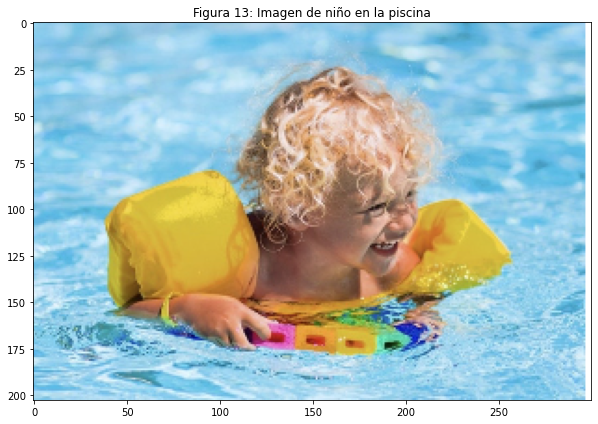
\includegraphics[width=\textwidth]{imagenes/PoissonImageEditing_cell_23_output_1.png}
        \caption{Imagen original sin seleccionar}
    \end{subfigure}
    \begin{subfigure}[t]{0.25\textwidth}
        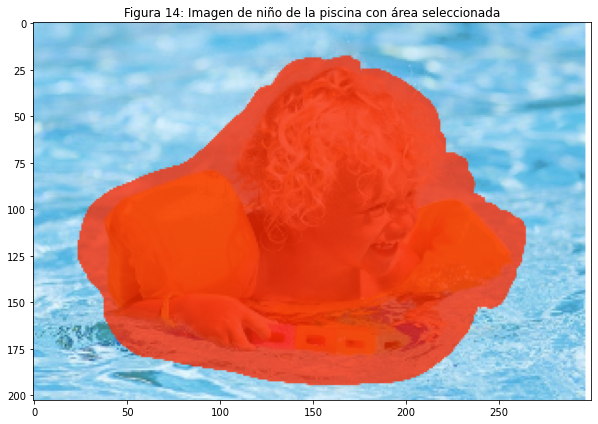
\includegraphics[width=\textwidth]{imagenes/PoissonImageEditing_cell_23_output_2.png}
        \caption{Región seleccionada $R$ en rojo}
    \end{subfigure}
    \begin{subfigure}[t]{0.25\textwidth}
       \centering
        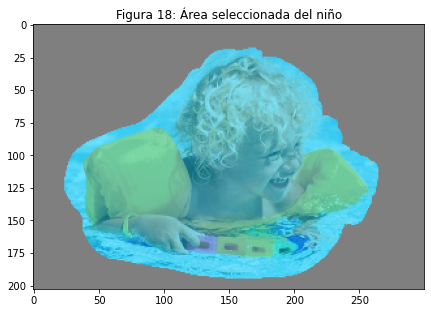
\includegraphics[width=\textwidth]{imagenes/PoissonImageEditing_cell_23_output_6.png}
        \caption{Visualización del conjunto de píxeles seleccionados por el algoritmo}
    \end{subfigure}
    \caption{Ejemplo de selección de regiones}
    \label{fig:ejemploSeleccionRegiones}
\end{figure}

Es necesario crear un sistema de selección de regiones para nuestro problema, es decir, lo que de manera teórica sería definir las regiones $\Omega$ y $S$. Para ello utilizamos el siguiente método: 

Se subirán dos imágenes, que gracias a la respectiva lectura con las funciones de opencv \texttt{Código 3}, las imágenes tendrán una estructura matricial de reales. Una de las imágenes leída será la original sin seleccionar el área, otra la que tiene el área seleccionada. Para indicar las regiones lo que se hará será cambiar el color de esa región. Puede encontrar un ejemplo en la figura \ref{fig:ejemploSeleccionRegiones}.  

Mostramos ejemplo en  \texttt{Código: 5} y \texttt{Código: 6}. 

La implementación del cálculo, en sección \texttt{Código: 4} se basa en que se ha cambiado el color de las región seleccionada.
Por lo que restando las matrices que representan las imágenes originales y la nueva, las entradas no nulas representa los píxeles seleccionados.

Este método supone un esfuerzo al que edita las imágenes: debe cambiar el color correctamente (es decir si lo hace coloreando esa región con un color, debe asegurarse de que ese color no está en ningún píxel de la zona. Para ello recomendamos usar algoritmos propios del programa de edición con que edite la foto.)

Otro problema ahora a hacer frente es dónde posicionar esos píxeles en la otra imagen, como veremos en apartados posteriores esto se hará gracia a movimientos rígidos.


\subsubsection{Movimientos rígidos} \label{section:movimientosRigidos}

Una consideración importante a tener en cuenta es que, una vez realizada la selección de la región a copiar, debe situarse correctamente dentro de la imagen destino. 
Esto implica realizar una transformación rígida (simetrías, traslaciones, rotaciones o composiciones de éstas) de la región, es decir a las coordenadas originales.   

El motivo por el que los movimientos elegidos son los rígidos es el siguiente: 

Son los únicos transformaciones que nos permiten establecer una biyección de la región seleccionada a la imagen destino, manteniendo la conexión y forma de la región. Cualquier otra deformaría la imagen o nos vería comprometidos a considerar tratamientos más complejos como una interpolación de píxeles.   

Es más, teniendo en cuenta los errores de redondeo y que las coordenadas de los píxeles de una imagen, aunque implementada, desaconsejamos introducir giros en la función de transformación. Si se desea realizar un insertado donde se ha girado la imagen aconsejamos girar antes la imagen source (ya sea con una herramienta de edición o multiplicando la imagen por una matriz de giro) obteniendo con ello una nueva imagen fuente en la que seleccionar la región concreta y ya aplicar nuestro algoritmo.  Y al igual que se ha procedido con el giro, si hay necesidad de alguna otra transformación no euclídea, será posible aplicarla de la misma manera. 

El convenio de vectores a los que aplicar las transformaciones será el clásico:  una tripleta $(x, y, w)$ donde $x$ es la coordenada del píxel en el eje X, $y$ es la coordenada del píxel en el eje Y y $w$ es la coordenada homogénea del punto (se supondrá $w=1$ para los píxeles de la imagen).

De esta forma se decide implementar una función, \texttt{GetMatrixTransformation} en la sección \texttt{Código: 10}. Los pasos seguidos en dicha función son los siguientes:

\begin{enumerate}
    \item Se calcula el centroide de la región en caso de no estar ya definido. Esto será necesario para transformaciones posteriores.
    \item Se calcula la matriz de traslación que posiciona el centroide de la región en el punto $(0, 0, 1)$.
    \item Se calcula la matriz de simetría y la matriz de rotación según los parámetros recibidos.
    \item Se calcula la matriz de traslación acorde a los parámetros recibidos.
    \item Se realiza la composición de transformaciones en el orden correcto.
\end{enumerate}

En cuanto a las matrices que definen las transformaciones anteriormente definidas, estas tienen la siguiente forma:

\begin{itemize}
    \item Matriz de traslación, denotada mediante $T_{x',y'}$ donde $x'$ denota el número de píxeles a trasladar en el eje X e $y'$ denota el número de píxeles a trasladar en el eje Y.
    $$T_{x',y'} = \begin{bmatrix}
    1 & 0 & x'\\
    0 & 1 & y'\\
    0 & 0 & 1
    \end{bmatrix}$$
    \item Matriz de rotación, denotada mediante $R_\alpha$ donde $\alpha$ denota el ángulo a rotar en grados.
    $$R_\alpha = \begin{bmatrix}
    \cos{\alpha} & -\sin{\alpha} & 0\\
    \sin{\alpha} & \cos{\alpha} & 0\\
    0 & 0 & 1
    \end{bmatrix}$$
    \item Matriz de simetría, denotada mediante $S$, que es una matriz de la forma:
    $$S = \begin{bmatrix}
    x_s & 0 & 0\\
    0 & y_s & 0\\
    0 & 0 & 1
    \end{bmatrix}$$
    Donde $x_s,y_s \in \{-1,1\}$ en función del eje sobre el que se realiza la simetría. El origen de los ejes donde se realiza la simetría es el centroide de  la región. 
\end{itemize}

\subsubsection{Medición de la bondad de las técnicas }

Un apartado interesante a tratar a la hora de afrontar técnicas de mezclado de imágenes es cómo medir la calidad de una solución y si es incluso posible plantearse una definición formal.   

Por el ámbito en que nos encontramos y diversidad de técnicas que afrontamos hemos optado por no utilizar ningún método numérico y basarnos tan solo en nuestro criterio como personas mediante inspección visual, que aunque subjetivo, no se nos ha ocurrido nada mejor. 

\subsubsection{Sobre la naturaleza de la región seleccionada}

Entre otras hipótesis, a nivel teórico $\Omega$ debe de ser un dominio euclídeo. Sin embargo, tras la discretización por cómo se define la ecuación a resolver  (\ref{eq:discretizada}) una selección de regiones disconexas no generaría ninguna incoherencia a nivel de cálculo y los resultados siendo consistentes. Esto se debe a que el sistema de ecuaciones resultante tendría forma de matriz bloque, es decir sería equivalente a tantos sistemas de ecuaciones como componentes disconexas hayan sido seleccionadas. 

De todas formas esto supondría un coste computacional, tanto de cálculo como de memoria importante y es por ello que no recomendamos que se seleccionen múltiples regiones disconexas a la vez. 

\newpage 
\section{Copiado de regiones conexas} 

\subsection{Descripción del problema}
El problema que se pretende resolver en esta sección es el siguiente:  Dada una región $R$ de píxeles seleccionados de una imagen $A$ se pretende copiar tal región en otra imagen $B$, de tal forma que $R$ en $B$ sea lo más verosímil posible.   

% Figuras playa 
\begin{figure}[h]
    \centering
    \begin{subfigure}[b]{0.3\textwidth}
        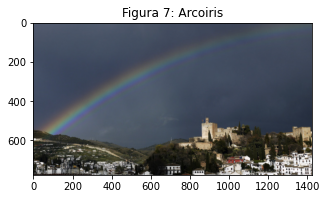
\includegraphics[width=\textwidth]{imagenes/PoissonImageEditing_cell_12_output_0.png}
        \caption{Imagen fuente $A$}
    \end{subfigure}
    \begin{subfigure}[b]{0.35\textwidth}
        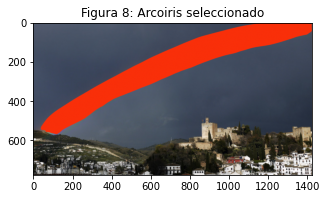
\includegraphics[width=\textwidth]{imagenes/PoissonImageEditing_cell_12_output_1.png}
        \caption{Región seleccionada $R$ en rojo}
    \end{subfigure}
    \begin{subfigure}[b]{0.3\textwidth}
       \centering
        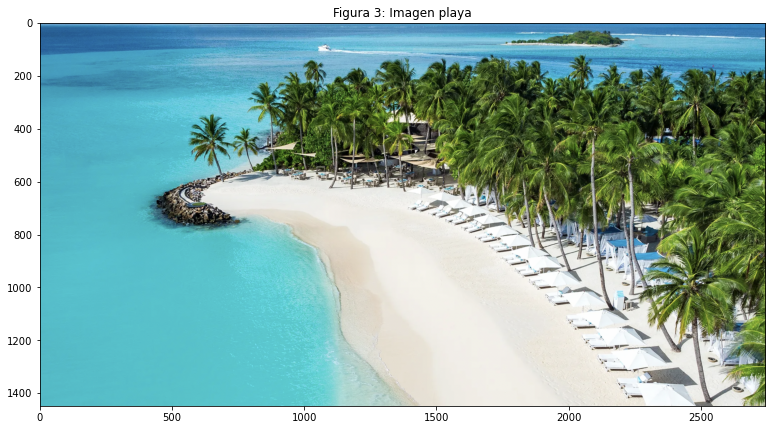
\includegraphics[width=\textwidth]{imagenes/PoissonImageEditing_cell_8_output_3.png}
        \caption{Imagen objetivo $B$}
    \end{subfigure}
    \caption{Elementos en un copiado de regiones}
    \label{fig:copiadoRegionesConexasArcoirisPlaya}
\end{figure}


Ejemplo de estos elementos son los que aparecen en la figura \ref{fig:copiadoRegionesConexasArcoirisPlaya}

\subsection{Aproximación directa}  

La solución trivial sería un clonado directo, pero esto en ocasiones no produce un resultado satisfactorio, véase por ejemplo la figura \ref{fig:copiadoRegionesConexasClonadoDirecto}

% Figura del oso en la piscina 
\begin{figure}[h]
    \centering
    \begin{subfigure}[t]{0.18\textwidth}
        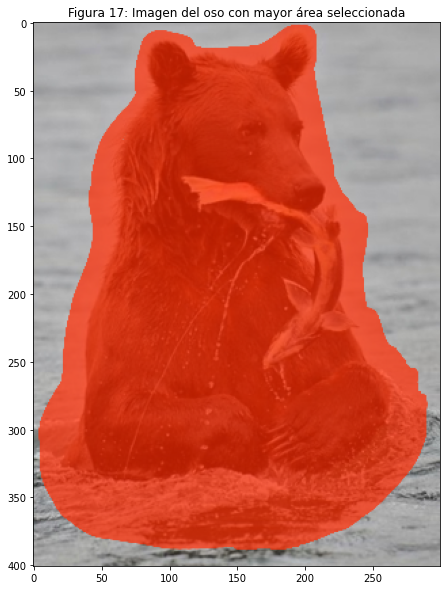
\includegraphics[width=\textwidth]{imagenes/PoissonImageEditing_cell_23_output_5.png}
        \caption{Región $R$ seleccionada de oso pardo}
    \end{subfigure}
    \begin{subfigure}[t]{0.36\textwidth}
        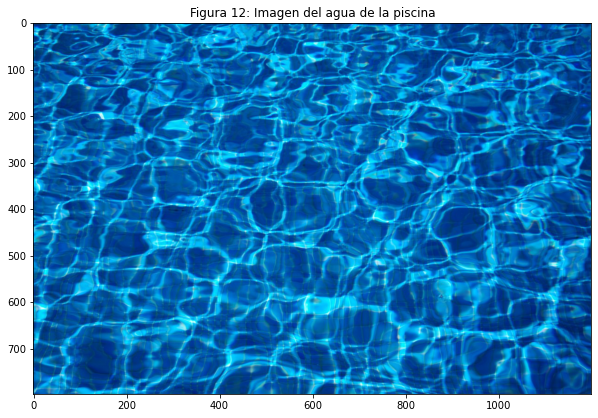
\includegraphics[width=\textwidth]{imagenes/PoissonImageEditing_cell_23_output_0.png}
        \caption{Imagen objetivo B de una piscina}
    \end{subfigure}
    \begin{subfigure}[t]{0.36\textwidth}
       \centering
        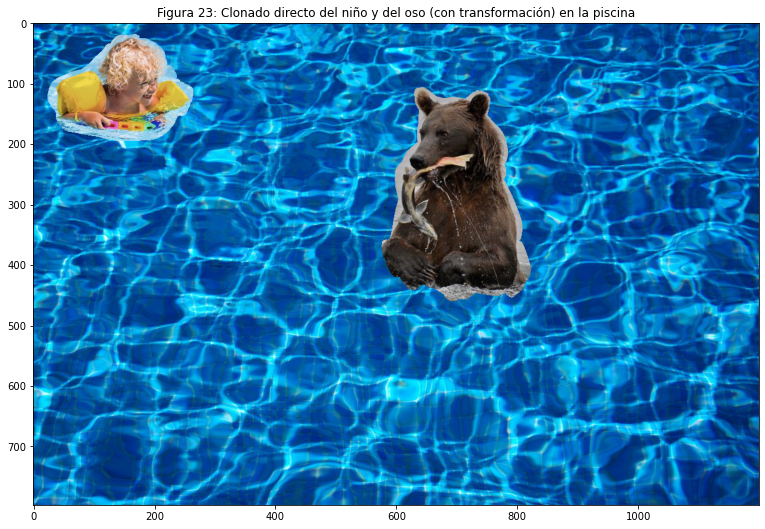
\includegraphics[width=\textwidth]{imagenes/PoissonImageEditing_cell_27_output_2.png}
        \caption{Resultado clonación copiado directo}
    \end{subfigure}
    \caption{Elementos y resultado de clonado directo}
    \label{fig:copiadoRegionesConexasClonadoDirecto}
\end{figure}

Surge con esto la técnica de \textit{seamless cloning} la cual nosotros hemos traducido como \textit{copiado prístino}.   

\subsection{Copiado prístino}\label{tecnica:copiadoPristino}

Notemos que al introducir el problema en la ecuación  (\ref{eq:eulerLagrange}) se hace referencia a un campo vectorial que no se explicita, la definición de éste será clave a lo largo del desarrollo de las técnicas.   

\subsubsection{Fundamento técnico}
Para el copiado prístino este campo será el gradiente de la imagen fuente esto es 

\begin{equation}
    \textbf{v} = \nabla g.
\end{equation}

que sustituyendo en (\ref{eq:condicionesBordeContinuo}) y aplicando la igualdad de que bajo estas hipótesis el gradiente de la divergencia de una función equivale al laplaciano de la función resulta:  

\begin{equation}
    \nabla f = \nabla g \text{ en } \Omega, \text{con condiciones en borde } f|_{\partial \Omega} = f^* | _{\partial \Omega}.
\end{equation}  

La implementación numérica, declarada en \texttt{Código 2} es la siguiente: 

\begin{equation}
   v_{p,q} = g_p - g_q  \text { si } p,q \in \Omega \quad \text{  ó   }\quad v_{p,q} = g_p - f_q \text{ si } q \in \partial \Omega,  p \in \Omega  
\end{equation}

\subsubsection{Resultados} 
% Ejemplo bueno de oso polar en la playa
Realizaremos una demostración de la técnica integrando el oso polar en el agua de mar que se muestran en la figura \ref{fig:copiadoPristinoElementosOsoPolarYMar}.   

%... Oso polar y playa:,Imagen de un oso polar y mar donde se quiere insertar
\begin{figure}[h]
    \centering
    \begin{subfigure}[b]{.45\textwidth}
        \centering
        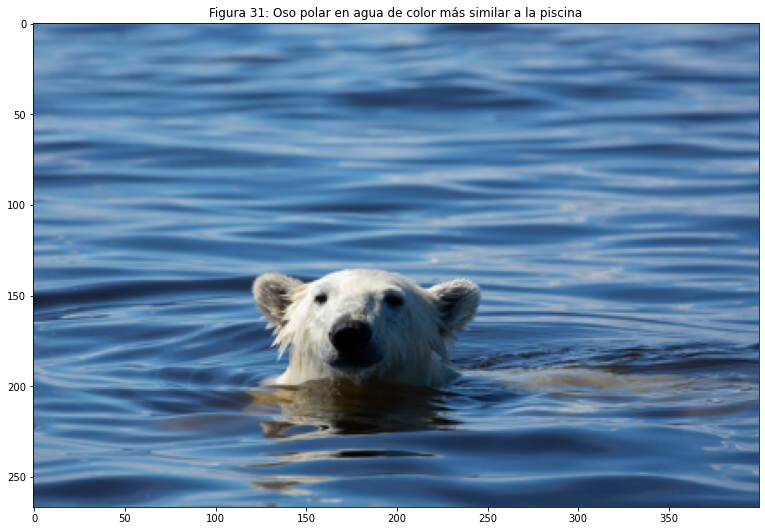
\includegraphics[width=\textwidth]{imagenes/PoissonImageEditing_cell_40_output_1.png}
        \caption{Imagen objetivo de oso polar a insertar}
    \end{subfigure}%
    \begin{subfigure}[b]{.45\textwidth}
        \centering
        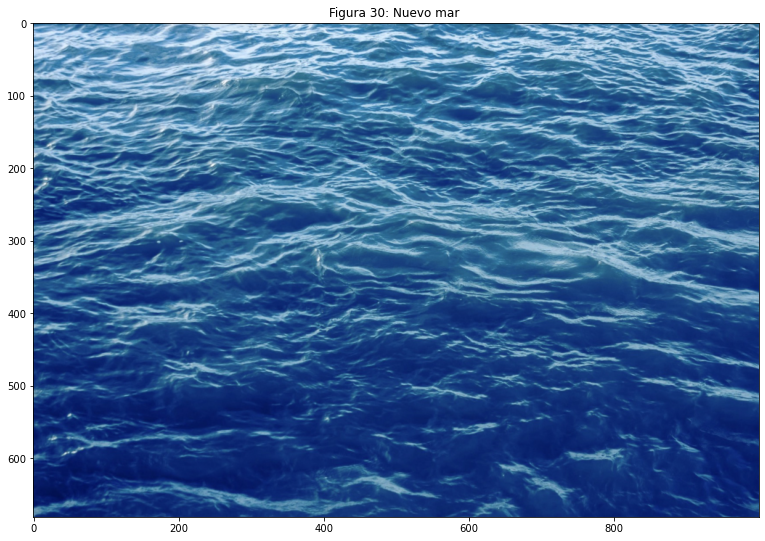
\includegraphics[width=\textwidth]{imagenes/PoissonImageEditing_cell_40_output_0.png}
        \caption{Imagen destino, mar}

    \end{subfigure}
    \caption{Imagen de un oso polar y mar donde se quiere insertar}
    \label{fig:copiadoPristinoElementosOsoPolarYMar}
\end{figure}

%... Oso polar y playa:,Imagen de un oso polar y mar donde se quiere insertar
\begin{figure}[h]
    \centering
    \begin{subfigure}[b]{.45\textwidth}
        \centering
        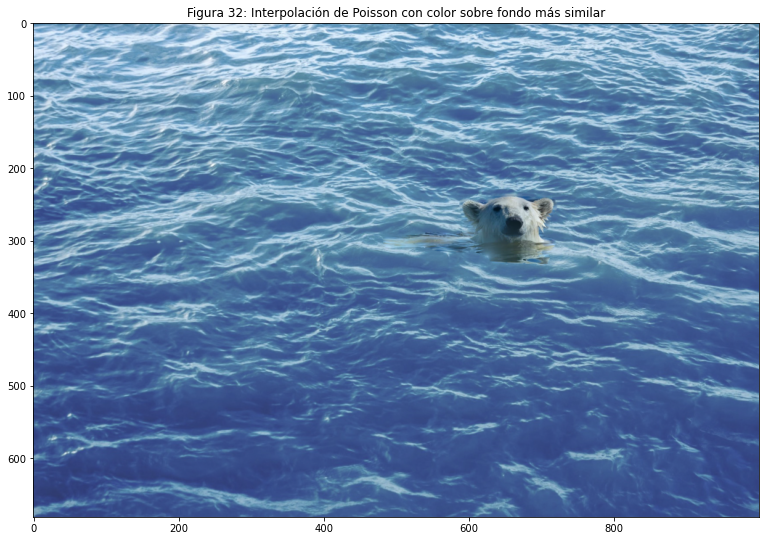
\includegraphics[width=\textwidth]{imagenes/PoissonImageEditing_cell_40_output_2.png}
        \caption{Copiado prístino del oso en región clara del mar}
        \label{fig:copiadoPristinoOsoPolar1}
    \end{subfigure}%
    \begin{subfigure}[b]{.45\textwidth}
        \centering
        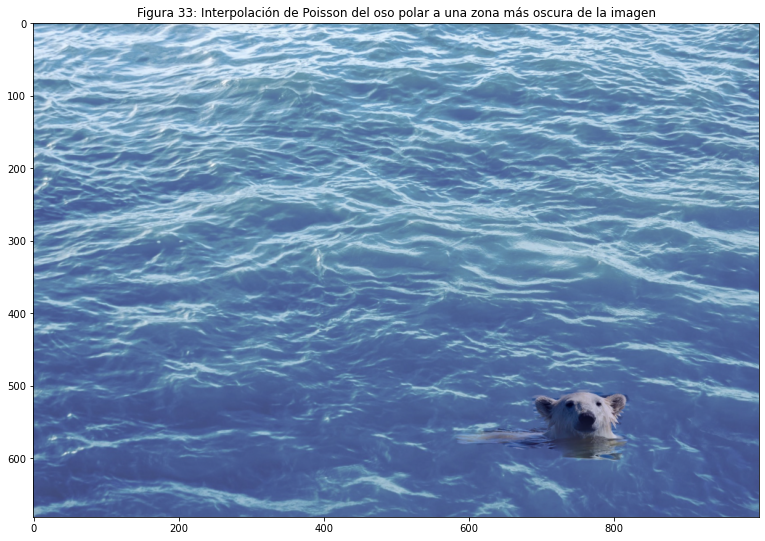
\includegraphics[width=\textwidth]{imagenes/PoissonImageEditing_cell_42_output_0.png}
        \caption{Resultado copiado prístino del oso en región oscura}
        \label{fig:copiadoPristinoOsoPolar2}
    \end{subfigure}
    \caption{Resultado de copiado prístino de oso en mar en distintas situaciones}
    \label{fig:copiadoPristinoOsoPolarYMar}
\end{figure}

Bajo una inspección visual puede comprobarse que los resultados del copiado prístino, mostrados en la figura \ref{fig:copiadoPristinoOsoPolarYMar} son plausibles de ser realidad. Puede observarse un cambios de luz en la cara del oso, siendo en la figura \ref{fig:copiadoPristinoOsoPolar1} más clara que  en  \ref{fig:copiadoPristinoOsoPolar2}.  

El motivo de esto reside, explicando de manera intuitiva, en que  algoritmo de copiado prístino basa
la intensidad de colores en las diferencias que encuentre en el borde la la región seleccionado y los píxeles de la imagen objetivo donde se sitúa tal borde.  
Es decir que en nuestro caso particular entiende que tiene que igualar el agua que bordea al oso con la de la posición del agua de mar de la imagen destino dónde se coloca; aplicando tal transformación al interior de la región a insertar.

\subsubsection{Ejemplos patológicos de la técnica de copiado prístino}
\label{SectionEjemploPatologicos}
Con el fin de evidenciar cómo se comporta la técnica de copiado prístino con los fondos y la necesidad de un borde similar en la región seleccionado y la imagen destino mostraremos más ejemplos. 

Tomaremos como \textbf{un primer ejemplo la inserción de un oso pardo en una piscina }, véanse en la figura  \ref{fig:copiadoPristinoOsoOscuroYPiscina}. 

\begin{figure}[h]
    \centering
    \begin{subfigure}[b]{.31\textwidth}
        \centering
        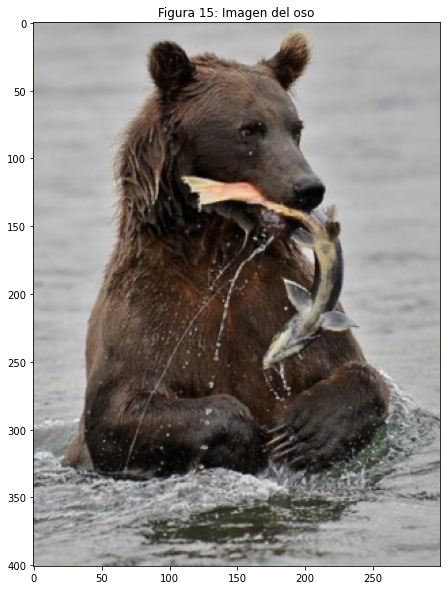
\includegraphics[width=\textwidth]{imagenes/PoissonImageEditing_cell_23_output_3.png}
        \caption{Imagen fuente oso pardo}
        \label{fig:cpOsoPArdo}
    \end{subfigure}%
    \begin{subfigure}[b]{.59\textwidth}
        \centering
        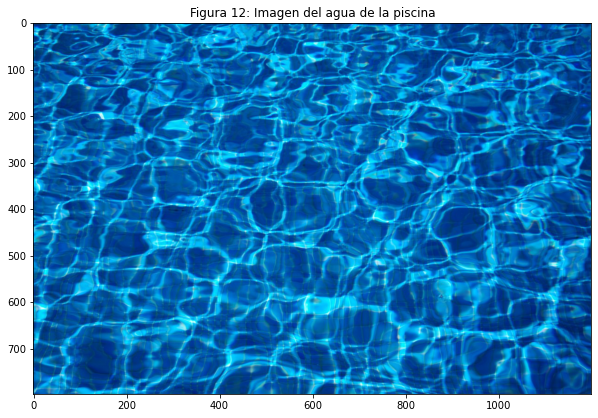
\includegraphics[width=\textwidth]{imagenes/PoissonImageEditing_cell_23_output_0.png}
        \caption{Imagen objetivo piscina}
        \label{fig:cpPiscina}
    \end{subfigure}
    \caption{Oso pardo y piscina }
    \label{fig:copiadoPristinoOsoOscuroYPiscina}
\end{figure}


\begin{figure}[h]
    \centering
    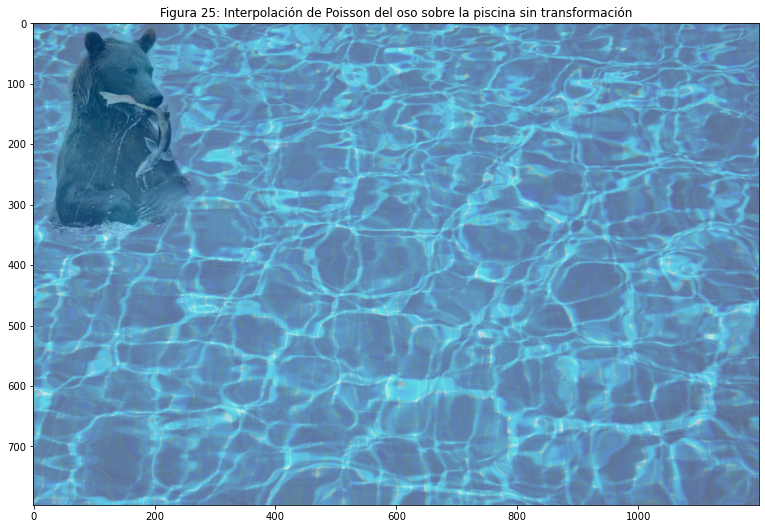
\includegraphics[width=.7\textwidth]{imagenes/PoissonImageEditing_cell_30_output_1.png}
    \caption{Inserción oso pardo en piscina con copiado prístino}
    \label{fig:cposopardo1}
\end{figure}


Obtenemos tras aplicar el copiado la imagen  de la figura \ref{fig:cposopardo1}. 

El resultado es indudablemente malo en lo que respecta a una inserción real, principalmente por los siguientes motivos:
\begin{enumerate}
    \item Se ha alterado el color del agua de la imagen objetivo, notése la diferencia entre las figuras \ref{fig:cpPiscina} y \ref{fig:cpOsoPArdo}. 
    \item El color actual del oso es demasiado azul para ser tomado como real. 
\end{enumerate}

Para dar explicación a esto debemos de tener presente la diferencia de color del agua que hay entre  \ref{fig:cpOsoPArdo} y la imagen  objetivo original \ref{fig:cpPiscina}. Explicado de forma filosófica, para el algoritmo todas las aguas son las mismas y la diferencia entre ellas es la luminosidad, luego al tratar de  \textit{corregir} tal diferencia provoca la distorsión cromática del oso comentada.    

Por otra parte, si partimos de la base de que el algoritmo de copiado prístino no altera los píxeles exteriores a la región destino ¿Por qué ha cambiado el color en  el cambio de color del agua del mar de la imagen resultado \ref{fig:cposopardo1}?  

Esto tiene dos motivos fundamentales, el primero es que como ya adelantábamos en la teoría subyacente se debe a que los valores posibles de de la solución buscada $f$ no están acotados, luego cualquier valor real es susceptible de darse. En nuestro caso, las grandes diferencias de colores en los fondos ha incrementado circunstancialmente el canal azul haciéndolo tomar valores fuera incluso del rango habitual. El segundo motivo es consecuencia de la técnica de pintado (ver en \texttt{Código 3}) , donde independientemente de los valores de la imagen estos se normalizan y reescalan dentro del rango $[0,1]$ y tras esto se muestra la imagen; como había valores fuera del rango el cambio de color es consecuencia de tal preprocesamiento.    

Esta conclusión ha sido fruto te los experimentos realizados en el apartado 3.8 del código que comprende las celdas \texttt{Código 14, ..., 18}. 

\begin{figure}[h]
    \centering
    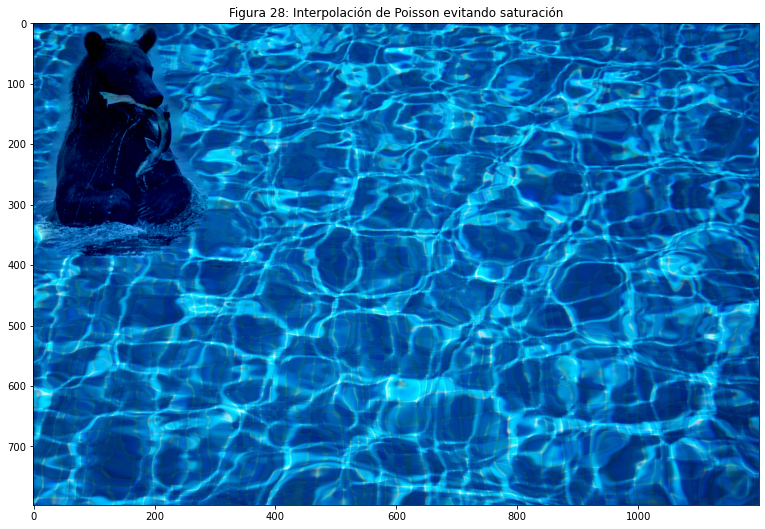
\includegraphics[width=.7\textwidth]{imagenes/PoissonImageEditing_cell_35_output_0.png}
    \caption{Oso evitando valores fuera de rango. }
    \label{fig:cposoSaturado}
\end{figure}

Puede observar en la figura \ref{fig:cposoSaturado} cómo se vería la imagen si tras el cálculo de $f$, transformáramos a $0$ los valores negativos y a $255$ los positivos.  
El oso está completamente saturado, dando como ya hemos comprobado en la figura \ref{fig:cposopardo1} el tono azul del oso. Por otra parte y como esperábamos el color del agua se ha mantenido igual.  

Otro experimento que realizamos en \texttt{Código 15, experimento 1} fue variar el margen el oso, no se notaron resultado concluyentes, lo cual es coherente con la teoría ya que el \textit{grosor} del borde es de un píxel. 



% Imagen de la playa con el arcoíris
\begin{figure}[h]
    \centering
    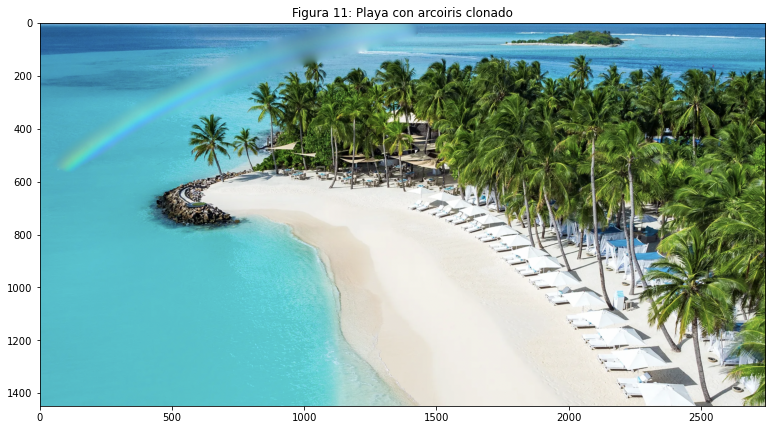
\includegraphics[width=.7\textwidth]{imagenes/PoissonImageEditing_cell_18_output_0.png}
    \caption{Inserción de un arcoíris en una playa Por técnica de copiado prístino}
    \label{fig:arcoirisCopiadoPristino}
\end{figure} 

% ejemplo de palmera sobre playa %%
Mostraremos ahora la influencia del fondo con un \textbf{segundo ejemplo en el que se mostrará la inserción de un arcoíris en una playa} aplicando el algoritmo a los elementos presentados en la figura  \ref{fig:copiadoRegionesConexasClonadoDirecto} se ha obtenido el siguiente resultado \ref{fig:arcoirisCopiadoPristino}.


Podemos observar en la figura \ref{fig:arcoirisCopiadoPristino} que el resultado en la zona próxima a la copa de las palmeras no ha sido muy bueno, trataremos más a fondo el motivo y solución en la subsección \ref{subsection:InsercionObjetosTransparente}. 



% Blanca trabajando hasta aquí 

\newpage

\section{Técnica de borrado de regiones}

\subsection{Fundamento, descripción y resultados}

Ahora se quiere eliminar fragmentos como las pintadas de la \textit{Figura \ref{fig:paredPintada}}.

La idea general aplicada en la celda \texttt{Código 47} consiste en clonar a la región de la pintada una zona limpia.  Además si el tamaño de la pintada es mayor que el de la región limpia, se debe de considerar repetir el proceso de clonado de manera iterativa. Esta concatenación da lugar a diferentes casuísticas  que hemos condensado en: 

\begin{enumerate}
    \item \textbf{Unión de resultados calculados en paralelo}. Todas las clonaciones se hacen partiendo de la imagen original y al final se \textit{pega} una región dentro de otra. 
    \item \textbf{Cálculo recursivo}. La imagen clonada es ahora la objetivo de la siguiente. 
\end{enumerate}

\begin{figure}[h]
    \centering
    \begin{subfigure}[t]{.3\textwidth}
        \centering
        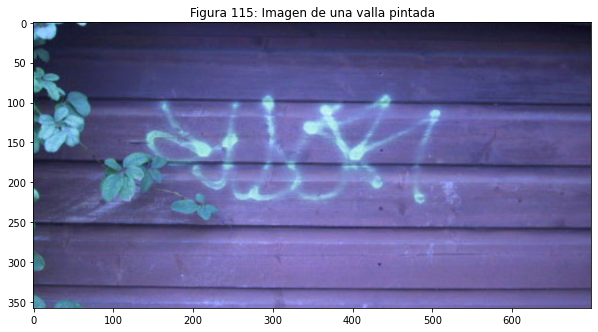
\includegraphics[width=\textwidth]{imagenes/PoissonImageEditing_cell_118_output_0.png}
        \caption{Imagen con pintadas}
        \label{fig:paredPintada}
    \end{subfigure}
    \centering
    \begin{subfigure}[t]{.3\textwidth}
        \centering
        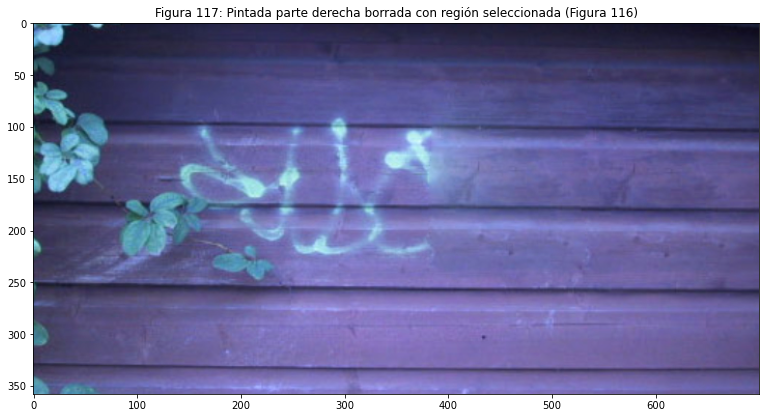
\includegraphics[width=\textwidth]{imagenes/PoissonImageEditing_cell_118_output_2.png}
        \caption{Borrado región derecha}
        \label{fig:borradoDerecho}
    \end{subfigure}
    \centering
    \begin{subfigure}[t]{.3\textwidth}
        \centering
        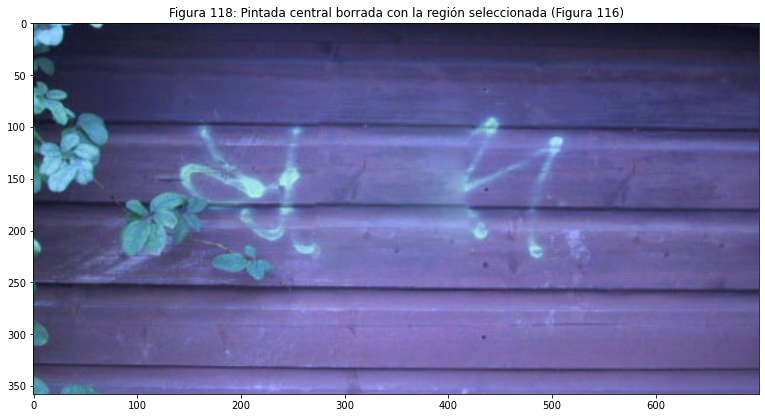
\includegraphics[width=\textwidth]{imagenes/PoissonImageEditing_cell_118_output_3.png}
        \caption{Borrado región central}
        \label{fig:borradoCentral}
    \end{subfigure}
    \centering
    \begin{subfigure}[t]{.3\textwidth}
        \centering
        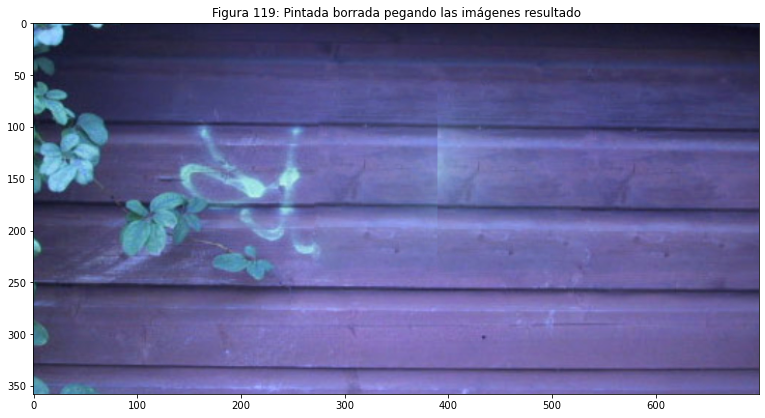
\includegraphics[width=\textwidth]{imagenes/PoissonImageEditing_cell_118_output_4.png}
        \caption{Unión de resultados}
        \label{fig:borradoUnion}
    \end{subfigure}
    \centering
    \begin{subfigure}[t]{.3\textwidth}
        \centering
        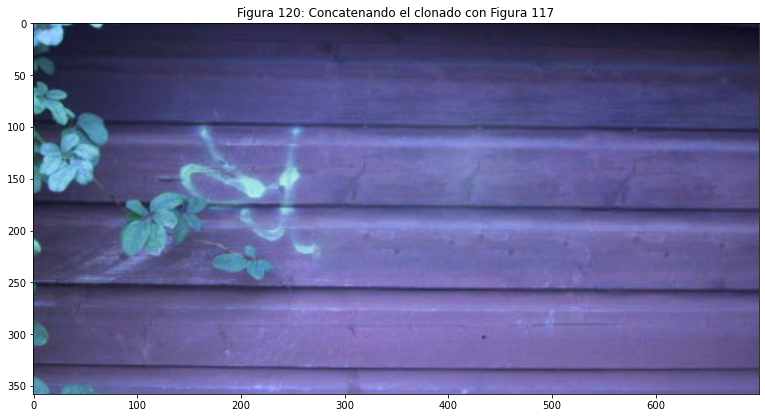
\includegraphics[width=\textwidth]{imagenes/PoissonImageEditing_cell_118_output_5.png}
        \caption{Borrado iterativo}
        \label{fig:borradoIterativo}
    \end{subfigure}
    \caption{Presentación de imagen de ejemplo y distintos borrados obtenidos}
    \label{fig:resultadosBorradoImágenes}
\end{figure}

Respecto al borrado de una región concreta, puede observarse en \textit{Figura \ref{fig:borradoDerecho}} y en \textit{Figura \ref{fig:borradoCentral}}, que el borrado funciona de una manera aceptable, presentando un peor acabado en las zonas en que los colores de la pintada son muy intensos. 

Respecto a la combinación de las imágenes, el método que calcula las figuras por separado y luego \textit{une} las imágenes no presenta resultados adecuados, ya que en la región límite hay un cambio brusco que da sensación de anti-naturalidad \textit{Figura \ref{fig:borradoUnion}}. Sin embargo el método iterativo \textit{Figura \ref{fig:borradoIterativo}} es el que consigue mejores resultados.

\subsection{Defectos del método y propuesta de soluciones}

Hemos observado dos defectos de este método:

\begin{enumerate}
    \item Como ya se ha comentado, en la regiones en que la pintaba presentaba más intensidad no se ha terminado de borrar del todo bien. Esto se debe a que la función de interpolación se aplica sobre el color de la imagen original. 
    \item Aparecen patrones de texturas en la imagen. 
\end{enumerate}

El defecto 2 se puede corregir con una selección manual de la regiones que parta de texturas diferentes. Para el primero  presentaremos un algoritmo nuevo original.

\subsection{Borrado de regiones por clonación opuesta}

La idea de este algoritmo subyace en la necesidad de eliminar la pintada total, aunque por su naturaleza  la intensidad de ésta sea mayor en regiones interiores de la selección. 

Explicaremos el método para el caso de las pintadas en la pared, pero puede observarse que es fácilmente generalizable la idea. 

Para ello: 

Denotemos como $I_0$ a la imagen original con la pintada a borrar, que es la región seleccionada $R$.
La idea consiste en clonar $R$  de la pared aplicando el movimiento rígido $T$, obteniendo con ello la imagen $I_1$. 
Sea $M$ la  diferencia $I_1 - I_0$, $M$ es una máscara que \textit{filosóficamente significa lo que hay que añadir a la pared para que aparezca la pintada} $R$.

La imagen $I_r$ que elimina la región $R$ se calcula como  $I_r = I_0 - T^{-1}(M)$.
 
Nótese que cuanto más parecido sea la superficie en la que se situa $R$ a la región que rodea $T(R)$ mejor será el resultado. 

La implementación puede observarse en la celda \texttt{Código 48} del código notebook.

\begin{figure}[h]
    \centering
    \begin{subfigure}[t]{.45\textwidth}
        \centering
        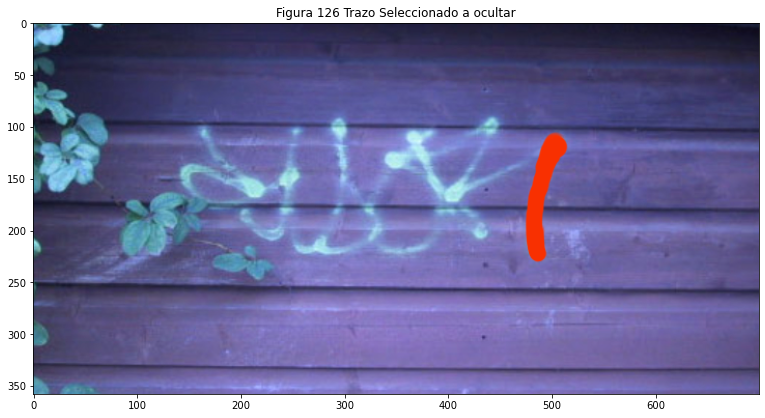
\includegraphics[width=\textwidth]{imagenes/PoissonImageEditing_cell_120_output_4.png}
        \caption{Región derecha a borrar}
        \label{fig:seleccionDerecha}
    \end{subfigure}
    \centering
    \begin{subfigure}[t]{.45\textwidth}
        \centering
        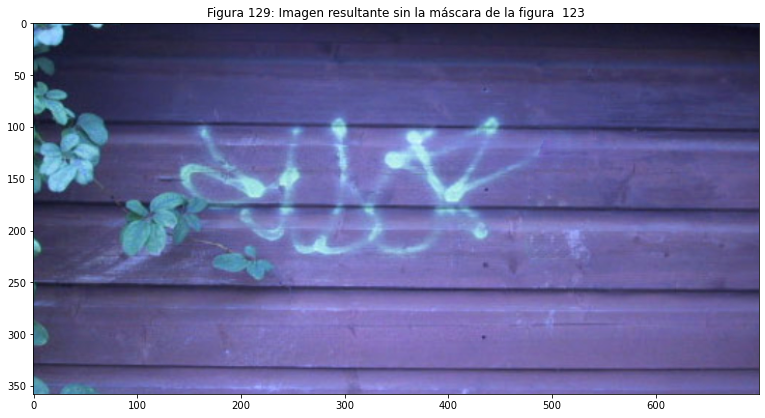
\includegraphics[width=\textwidth]{imagenes/PoissonImageEditing_cell_120_output_7.png}
        \caption{Borrado región derecha mediante clonación opuesta}
        \label{fig:borradoDerechoOpuesto}
    \end{subfigure}
    \centering
    \begin{subfigure}[t]{.45\textwidth}
        \centering
        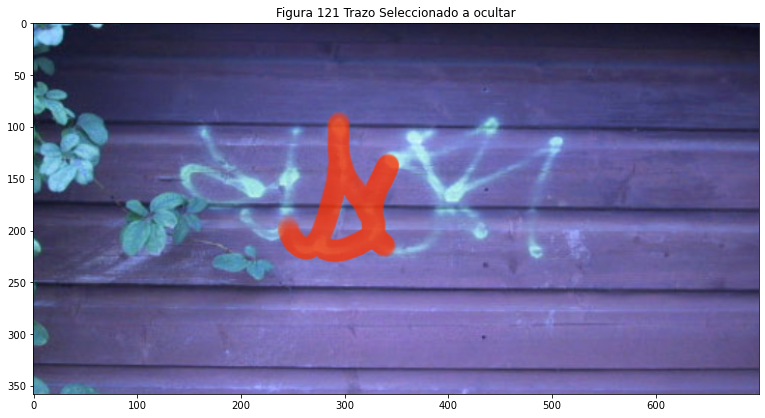
\includegraphics[width=\textwidth]{imagenes/PoissonImageEditing_cell_120_output_0.png}
        \caption{Región central a borrar}
        \label{fig:seleccionCentral}
    \end{subfigure}
    \centering
    \begin{subfigure}[t]{.45\textwidth}
        \centering
        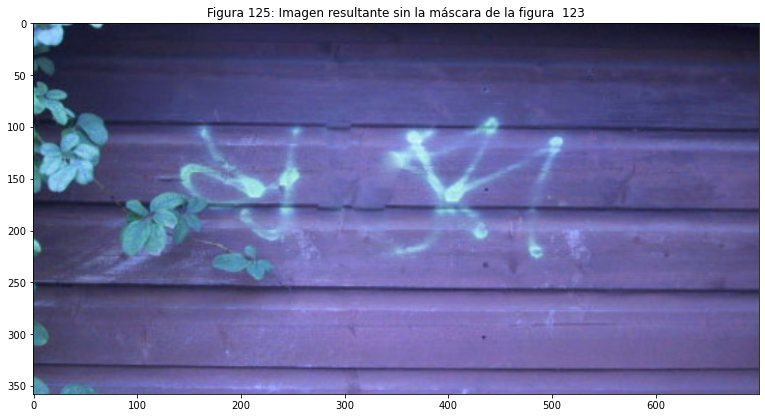
\includegraphics[width=\textwidth]{imagenes/PoissonImageEditing_cell_120_output_3.png}
        \caption{Borrado región central mediante clonación opuesta}
        \label{fig:borradoCentralOpuesto}
    \end{subfigure}
    \caption{Resultados obtenidos mediante el uso de borrado por clonación opuesta}
    \label{fig:resultadosClonacionOpuesta}
\end{figure}

Podemos observar que en el caso de eliminar la región que aparece en la \textit{Figura \ref{fig:seleccionDerecha}} el resultado obtenido en \textit{Figura \ref{fig:borradoDerechoOpuesto}} ha sido un éxito.   

Sin embargo para la región de la \textit{Figura \ref{fig:seleccionCentral}}, su resultado \textit{Figura \ref{fig:resultadosClonacionOpuesta}} no ha sido el deseado debido principalmente a la hendidura de la pared;que al no ser totalmente horizontal, y estar la región limpia suficientemente lejos de las coordenadas originales de la región seleccionada, no aparece en los mismo píxeles que en $R$, dando una sensación de distorsión.    

Esto se podría arreglar realizando un clonado iterativo de derecha a izquierda, como el del experimento 2 de la eliminación regiones anterior, de esta manera se iría \textit{limpiando la pared} y estas nuevas regiones podrían utilizarse para aplicar el método de la máscara, reduciendo con ello el error por la posición de la hendidura. Lo que supondría de nuevo ir seleccionando trazo lo suficientemente pequeños. 

\subsection{Conclusiones}

Tanto el método (1)  que propone el artículo \cite{poissonImageEditing} de clonar regiones limpias como el nuestro (2) requieren de un trabajo manual de selección de la región. La idoneidad de uno frente a otro puede provenir de: 

\begin{enumerate}
    \item Tamaño y forma de la región a eliminar. 
    \item Tiempo que se quiera dedicar a la eliminación de la región. 
    \item Nivel de perfección que se quiera alcanzar. 
\end{enumerate}

Ya que hemos visto que el método (2) alcanza mejores resultado si se hace con más paciencia, pero que con (1) con tan solo una región limpia seleccionada hemos conseguido eliminar más región.

\newpage

\section{Técnica de intercambio de características}

\subsection{Fundamento y descripción}

Utilizando la técnica de copiado prístino vamos a intercambiar las características de dos objetos; en nuestro caso concreto porosidad y manchas entre una manzana y una naranja (Ver figura \ref{fig:imagenIntercambioCaracterísticas}). Para ello será necesario: 

\begin{enumerate}
    \item Seleccionar independientemente las regiones de la pera y la naranja y luego aplicarlas intercambiadas. Debe de cuidarse en la selección que la región seleccionada en una fruta no exceda el tamaño de la otra.
    \item Cálculo de la traslación necesaria, se realizo en base a una translación observando los ejes de las imágenes. 
    \item Cálculo de los respectivos clonados.
    \item Se combinan las imágenes de de los respectivos clonados copiando los píxeles de una en otra. 
\end{enumerate}

\subsection{Resultados}

Los resultados obtenidos son los mostrados en la figura \ref{fig:resultadosIntercambioCaracteristicas} e implementados en la celda \texttt{Código 24} del código notebook.

\begin{figure}[h]
    \centering
    \begin{subfigure}[t]{.37\textwidth}
        \centering
        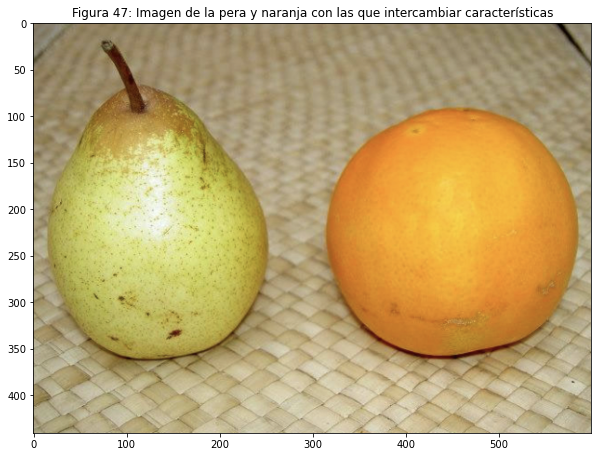
\includegraphics[width=\textwidth]{imagenes/PoissonImageEditing_cell_61_output_0.png}
        \caption{Imagen inicial}
        \label{fig:imagenIntercambioCaracterísticas}
    \end{subfigure}
    \centering
    \begin{subfigure}[t]{.37\textwidth}
        \centering
        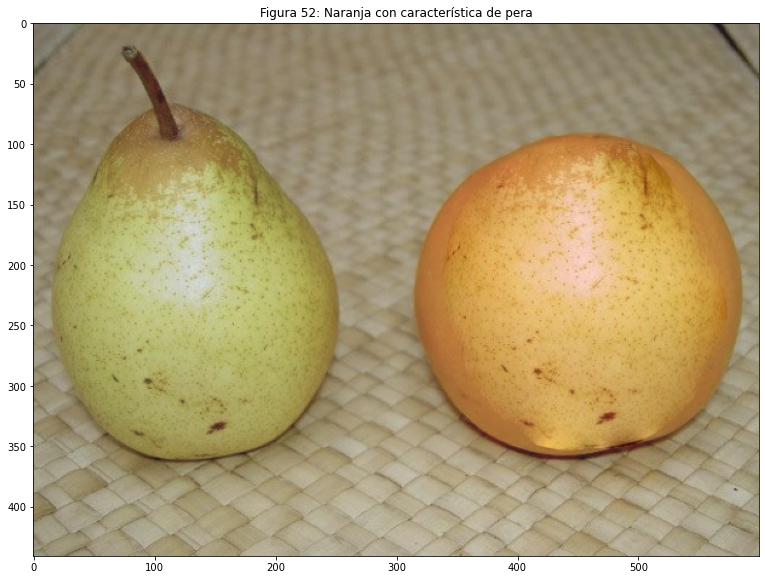
\includegraphics[width=\textwidth]{imagenes/PoissonImageEditing_cell_61_output_5.png}
        \caption{Naranja con característica de pera}
        \label{fig:naranjaAperada}
    \end{subfigure}
    \centering
    \begin{subfigure}[t]{.37\textwidth}
        \centering
        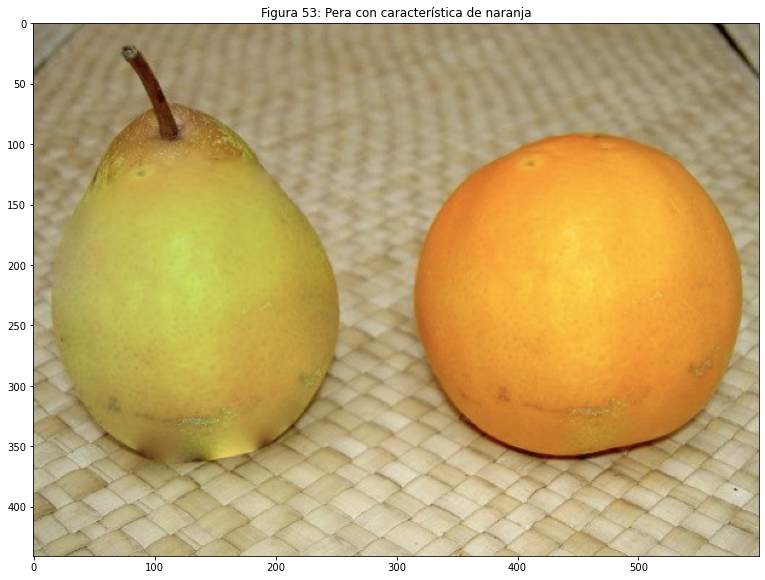
\includegraphics[width=\textwidth]{imagenes/PoissonImageEditing_cell_61_output_6.png}
        \caption{Pera con característica de naranja}
        \label{fig:peraAnaranjada}
    \end{subfigure}
    \centering
    \begin{subfigure}[t]{.37\textwidth}
        \centering
        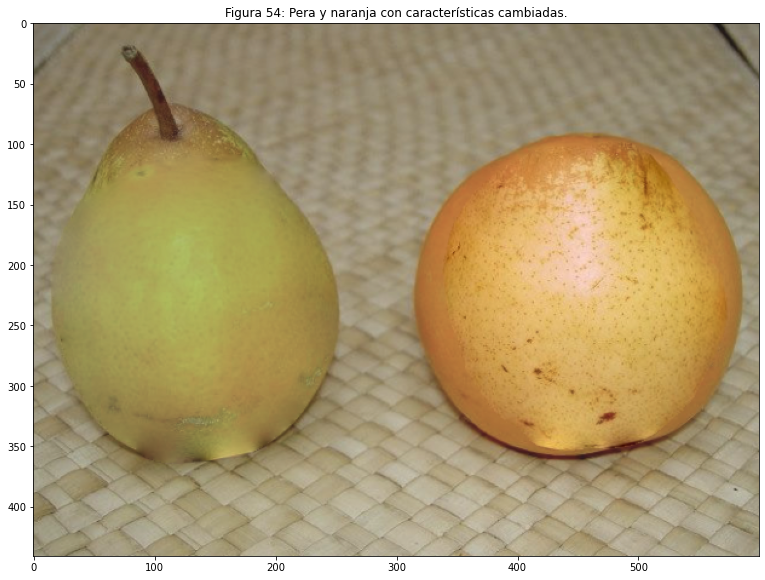
\includegraphics[width=\textwidth]{imagenes/PoissonImageEditing_cell_61_output_7.png}
        \caption{Intercambio de características}
        \label{fig:intercambioCaracteristicas}
    \end{subfigure}
    \caption{Resultados obtenidos mediante la técnica de intercambio de características}
    \label{fig:resultadosIntercambioCaracteristicas}
\end{figure}

\subsection{Conclusiones}

A priori, el resultado \textit{Figura \ref{fig:intercambioCaracteristicas}} es el buscado: una pera porosa y una naranja moteada.   

Sin embargo tiene los siguientes defectos: 

\begin{enumerate}
    \item \textbf{Existencia de regiones sin intercambiar características}. Esto era de esperar ya que las regiones seleccionada no tenían las misma forma. Para solventar este problema proponemos dos posibles soluciones:
    \begin{itemize}
        \item Aumentar por interpolación el tamaño de la imagen de la que se seleccionan características  y de ahí seleccionar los puntos que tengan la forma buscada de la otra fruta.
        \item Aumentar la región seleccionada a partir de repetirla, creando un mosaico.   
    Todas estas soluciones tienen en común una exigencia por parte del que prepara las imágenes, por no verle interés técnico no las hemos realizado.
    \end{itemize}
    \item \textbf{Problemas en la luminosidad}. Es evidente al ojo humano que la luz que tienen no es la que le corresponde. Sobretodo en las zonas inferiores \textit{Figura \ref{fig:intercambioCaracteristicas}}. Una posible solución sería preprocesar la imagen eliminan o suavizando los reflejos y luminosidad de esta manera ya no se mostrarían en la imagen. Si se precisara de tener reflejos estos podrían seleccionarse en un paso previo y añadirse nuevamente  utilizando el mezclado de Poisson ya implementado.
\end{enumerate}

\newpage

\section{Técnica de intercambio de color}

\subsection{Fundamento y descripción}

Para evidenciar la necesidad del uso de esta técnica se parte del intento de transferencia de características entre la pera de la sección anterior y una manzana roja. Dichas imágenes se pueden observar en \textit{Figura \ref{fig:manzanaPeraIntercambioCaracteristicas}}.

\begin{figure}[h]
    \centering
    \begin{subfigure}[t]{.33\textwidth}
        \centering
        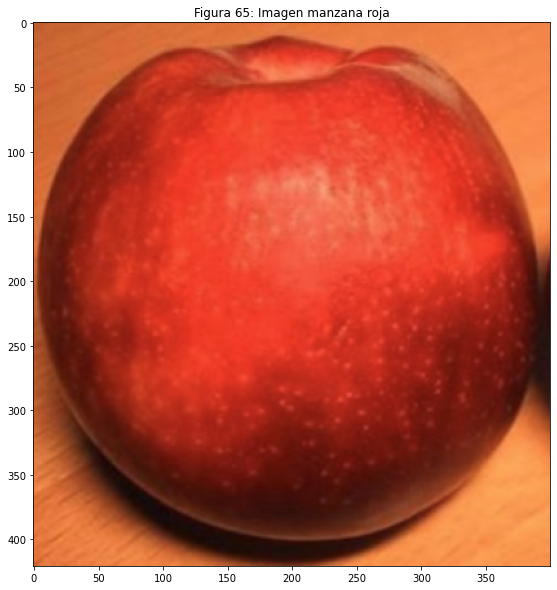
\includegraphics[width=\textwidth]{imagenes/PoissonImageEditing_cell_77_output_0.png}
        \caption{Manzana}
        \label{fig:manzanaIntercambioColor}
    \end{subfigure}
    \centering
    \begin{subfigure}[t]{.33\textwidth}
        \centering
        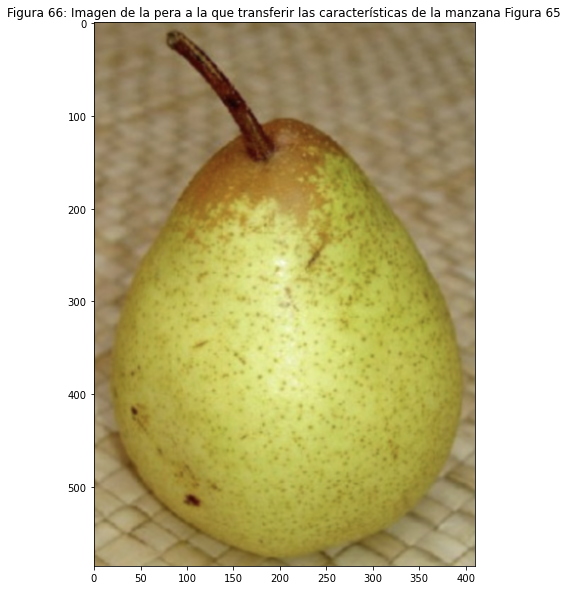
\includegraphics[width=\textwidth]{imagenes/PoissonImageEditing_cell_77_output_1.png}
        \caption{Pera}
        \label{fig:peraIntercambioColor}
    \end{subfigure}%
    \centering
    \begin{subfigure}[t]{.24\textwidth}
        \centering
        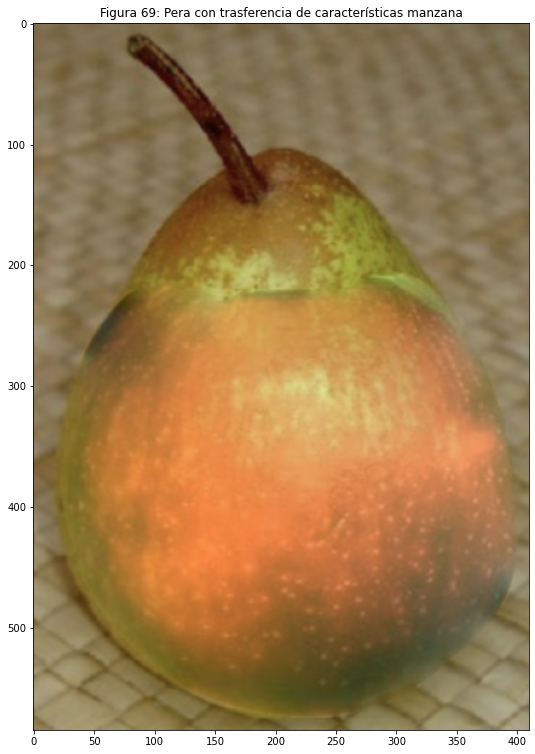
\includegraphics[width=\textwidth]{imagenes/PoissonImageEditing_cell_77_output_4.png}
        \caption{Intercambio de características}
        \label{fig:intercambioManzanaPera}
    \end{subfigure}
    \caption{Intercambio de características entre manzana y pera}
    \label{fig:manzanaPeraIntercambioCaracteristicas}
\end{figure}

Podemos observar en la \textit{Figura \ref{fig:intercambioManzanaPera}} que el resultado no ha sido tan bueno con en la transferencia de características de la \textit{Figura \ref{fig:intercambioCaracteristicas}}. Esto es debido a que la transferencia de color distorsiona el resultado. Para solucionar dicho defecto se realizará un clonado monocromático de la imagen fuente.Para ello se ha implementado la función \textit{ToMonochrome} en \texttt{Código 31} que no hace más que devolver una imagen monocromática pero de tres canales idénticos. Esta salida es necesaria ya que la función \textit{MultipleChannelDiscretePoissonSolverTransformed} (implementada en \texttt{Código 17}) necesita para el cálculo de la clonación una imagen de entrada de tres canales. 

\subsection{Resultados}

Los resultados presentados a continuación, \textit{Figura \ref{fig:manzanaPeraIntercambioMono}}, se encuentran implementados en la celda \texttt{Código 32} del código notebook.

\begin{figure}[h]
    \centering
    \begin{subfigure}[t]{.45\textwidth}
        \centering
        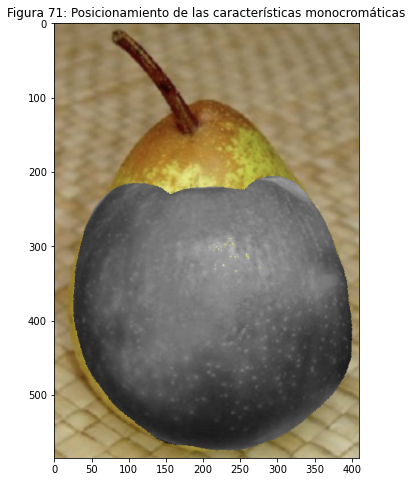
\includegraphics[height=5cm]{imagenes/PoissonImageEditing_cell_80_output_0.png}
        \caption{Posicionamiento de características}
        \label{fig:posCaracteristicasMono}
    \end{subfigure}
    \centering
    \begin{subfigure}[t]{.45\textwidth}
        \centering
        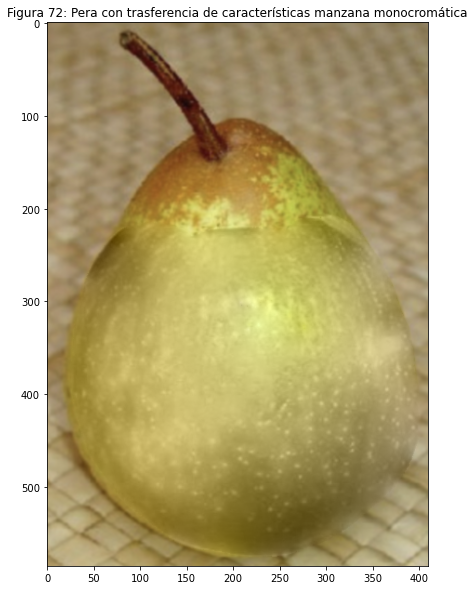
\includegraphics[height=5cm]{imagenes/PoissonImageEditing_cell_80_output_1.png}
        \caption{Transferencia de características monocromática}
        \label{fig:intercambioMonoPeraManzana}
    \end{subfigure}%
    \caption{Resultados de transferencia de características monocromática}
    \label{fig:manzanaPeraIntercambioMono}
\end{figure}

\subsection{Conclusiones}

Puede observarse en \textit{Figura \ref{fig:posCaracteristicasMono}} cómo se van a aplicar los píxeles de la imagen en escala de grises.  En la \textit{Figura \ref{fig:intercambioMonoPeraManzana}} aparece el resultado final, como vemos una transferencia de características mejor que la aportada en la \textit{Figura \ref{fig:intercambioManzanaPera}} en la que se transferían colores. El resultado podría haber sido mejor si se hubiera seleccionado con más cuidado las regiones de la manzana a trasferir \textit{Figura \ref{fig:manzanaIntercambioColor}}, ya que como vemos en la región de píxeles $[0,150] \times [200, 300]$ Las sombras de esa región no encajan del todo con la parte superior de la pera. 

\subsubsection{¿Por qué la transferencia monocromática ha sido clave?}

\begin{figure}[h]
    \centering
    \begin{subfigure}[t]{.45\textwidth}
        \centering
        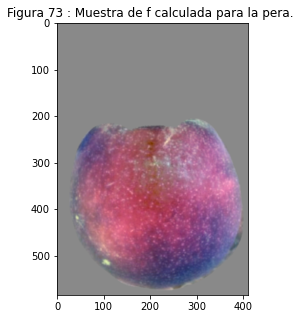
\includegraphics[height=5cm]{imagenes/PoissonImageEditing_cell_82_output_1.png}
        \caption{Muestra de f calculada para la pera}
        \label{fig:muestraFExperimento}
    \end{subfigure}
    \centering
    \begin{subfigure}[t]{.45\textwidth}
        \centering
        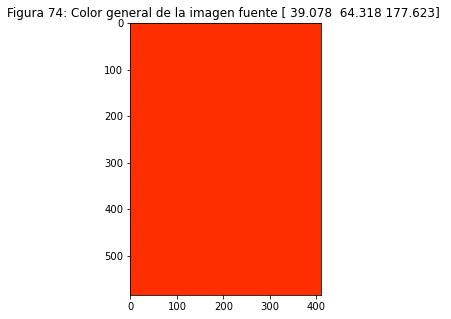
\includegraphics[height=5cm]{imagenes/PoissonImageEditing_cell_82_output_3.png}
        \caption{Color general de la imagen fuente}
        \label{fig:colorGeneralExperimento}
    \end{subfigure}%
    \caption{Resultados obtenidos en experimento asociado a \texttt{Código 33}}
    \label{fig:manzanaPeraIntercambioMono}
\end{figure}

Puede observarse en \textit{Figura \ref{fig:muestraFExperimento}} que el resultado de la interpolación $f$ de la transferencia de características con color de una manzana a una pera \textit{Figura \ref{fig:intercambioManzanaPera}} resulta una máscara roja. 

Para su cálculo se ha restado la imagen resultante de la interpolación \textit{Figura \ref{fig:intercambioManzanaPera}} con la objetivo \textit{Figura \ref{fig:peraIntercambioColor}}. 

Además, el \textbf{Cuadro \ref{table:2}} recoge un análisis numérico de  $f$ \textit{Figura \ref{fig:muestraFExperimento}} en el que gracias a la columna media se aprecia una tendencia general a potenciar el canal rojo y disminuir el azul y el verde. 

Para conocer el motivo de esto, debemos recordar que para el cálculo de transferencia se utiliza el campo de vectores guías (2), que recordemos que era el gradiente de la imagen fuente, y que se computaba como la diferencia entre píxeles vecinos. El problema está en que si aplicamos canal por canal de la  imagen fuente cromática, ésta, si tiene canales con cambios \textit{más intensos} respecto a otros, aumentará la intensidad de ese canal en el resultado de la interpolación, dando lugar a resultados como \textit{Figura \ref{fig:intercambioManzanaPera}}. 

 En nuestro caso vemos que esta situación se da, observando la \textbf{Cuadro \ref{table:1}} el canal rojo es el que presenta mayor intensidad general (media píxeles),  mayor cambio entre ellos (mayor varianza) y además estos saltos tienen el potencial de ser más grandes (valor mínimo píxeles). 

 A partir de la media, en la \textit{Figura \ref{fig:colorGeneralExperimento}} puede apreciarse ese color rojizo general de la imagen fuente. 

Por todo esto al realizar un ajuste monocromático, no se potenciará un canal frente a otro, si no que todos reflejarán características de textura. 

Los resultados de la salida de la celda \texttt{Código 33} se recogen en las siguientes tablas:

\begin{table}[h!]
\centering
\begin{tabular}{|| c ||c c c c||} 
 \hline
 Canal & Media píxeles & Varianza & Valor mínimo píxeles & Valor máximo píxeles \\ [0.5ex] 
 \hline\hline
 1 (azul) & 39.078 & 432.954 & 1 & 115 \\ 
 2 (verde) & 64.318  & 1356.462 & 2 & 160 \\
 3 (rojo) & 177.623 & 3287.625 & 17 & 243 \\ [1ex] 
 \hline
\end{tabular}
\caption{Resultados de la experimentación en canales  manzana realizada en \texttt{Código 33}.}
\label{table:1}
\end{table}

\begin{table}[h!]
\centering
\begin{tabular}{|| c ||c c c c||} 
 \hline
 Canal & Media píxeles & Varianza & Valor mínimo píxeles & Valor máximo píxeles \\ [0.5ex] 
 \hline\hline
 1 (azul) & -4.858 & 314.933 & -134.126 & 70.518 \\ 
 2 (verde) & -19.131  & 715.734 & -92.59 & 98.588 \\
 3 (rojo) & 6.615 & 674.034 & -95.236 & 114.838 \\ [1ex] 
 \hline
\end{tabular}
\caption{Parámetros observados en la máscara f que se aplica de traslación de características manzana sobre pera \texttt{Código 33}.}
\label{table:2}
\end{table}

Nota: Se ha incluido en el experimento de la imagen de la  manzana \textit{Figura \ref{fig:manzanaIntercambioColor}} el color de fondo, entendemos que puede hacer fluctuar los resultados, pero por ser su área considerablemente menor que la de la imagen fuente, pensamos que los resultados no afectarán en demasiado.

\subsubsection{Qué podemos aprender de la transferencia monocromática}

Acabamos de comprobar cómo el color de la imagen de interpolación afecta sensiblemente a los resultados, es por tanto lícito plantearse si modificar su valor a posteriori conduciría a mejores resultados, ya que como podemos ver en la \textit{Figura \ref{fig:muestraFExperimento}} el resultado no es del todo bueno porque el salto de color es demasiado. Es por ello que rebajaremos el color de $f$ multiplicándolo con un coeficiente.

\begin{figure}[h]
    \centering
    \begin{subfigure}[t]{.3\textwidth}
        \centering
        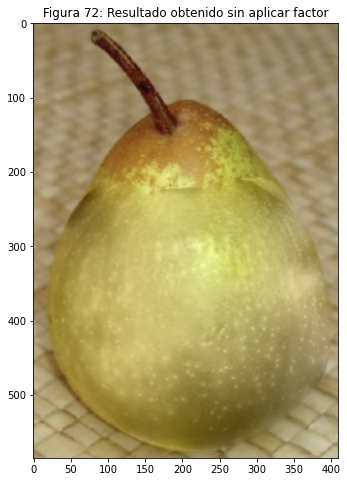
\includegraphics[height=5cm]{imagenes/PoissonImageEditing_cell_84_output_0.png}
        \caption{Sin aplicación de factor}
        \label{fig:noAplicacionFactor}
    \end{subfigure}
    \centering
    \begin{subfigure}[t]{.3\textwidth}
        \centering
        \captionsetup{justification=centering}
        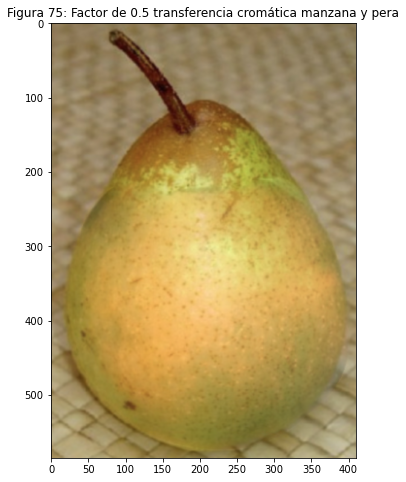
\includegraphics[height=5cm]{imagenes/PoissonImageEditing_cell_84_output_1.png}
        \caption{Factor de 0.5 en transferencia cromática}
        \label{fig:factor0.5Cromatica}
    \end{subfigure}%
    \centering
    \begin{subfigure}[t]{.3\textwidth}
        \centering
        \captionsetup{justification=centering}
        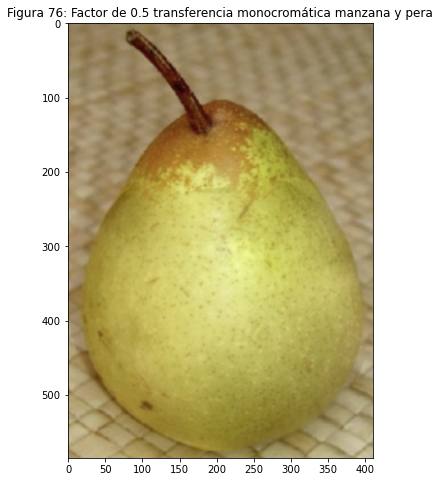
\includegraphics[height=5cm]{imagenes/PoissonImageEditing_cell_84_output_2.png}
        \caption{Factor de 0.5 en transferencia monocromática}
        \label{fig:factor0.5Mono}
    \end{subfigure}
    \centering
    \begin{subfigure}[t]{.3\textwidth}
        \centering
        \captionsetup{justification=centering}
        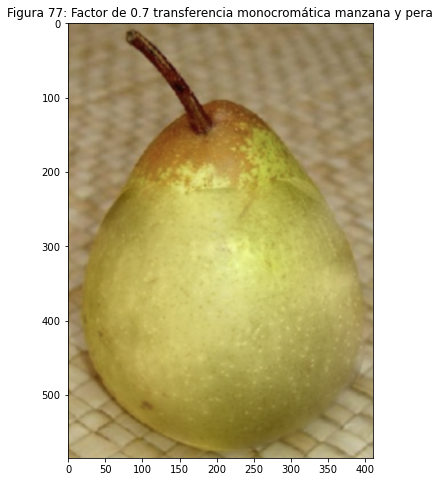
\includegraphics[height=5cm]{imagenes/PoissonImageEditing_cell_84_output_3.png}
        \caption{Factor de 0.7 en transferencia cromática}
        \label{fig:factor0.7Mono}
    \end{subfigure}%
    \centering
    \begin{subfigure}[t]{.3\textwidth}
        \centering
        \captionsetup{justification=centering}
        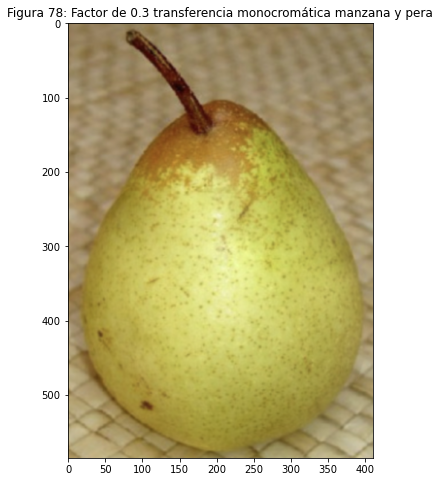
\includegraphics[height=5cm]{imagenes/PoissonImageEditing_cell_84_output_4.png}
        \caption{Factor de 0.3 en transferencia cromática}
        \label{fig:factor0.3Mono}
    \end{subfigure}
    \centering
    \caption{Resultados de la aplicación de varios factores en las transferencias de características}
    \label{fig:aplicacionFactoresIntercambio}
\end{figure}

Como podemos observar en \textit{Figura \ref{fig:factor0.5Cromatica}}  y \textit{Figura \ref{fig:factor0.5Mono}} los resultados han disminuido la distorsión de color aunque relajado la trasferencia de características. Quizás esa combinación lineal debería aplicarse en el cálculo de la ecuación de Poisson en lugar de antes. Sin embargo, en  \textit{Figura \ref{fig:factor0.3Mono}}, donde se ha relajado demasiado el color ($0.3$), se puede ver que la transferencia de características es inapreciable. En la  \textit{Figura \ref{fig:factor0.7Mono}} con un coeficiente de $0.7$ la transferencia se mantiene, pero la aberración de color sigue siendo notable. 

\newpage

\section{Técnica de mezcla de gradientes} \label{tecnica:mezcladoDeGradiente}

\subsection{Fundamento y descripción}

Es fácil ver que con la herramienta de copiado prístino (sección \ref{tecnica:copiadoPristino}), la información de la región interior $\Omega$ de la imagen destino no se tiene en cuenta a la hora de realizar la inserción. Es decir, no se tiene en cuenta la función $f^*$ en el cómputo de los píxeles de la región $\Omega$. Sin embargo, en casos concretos, como regiones que no sean simplemente conexas, el copiado prístino produce distorsiones por la falta de información ya mencionada, haciendo interesante mezclar la información de la imagen destino, $f^*$, y de la imagen destino, $g$. Por ejemplo, este efecto es interesante a la hora de insertar objetos con agujeros u objetos parcialmente transparentes.

Una posible aproximación inicial sería considerar el vector guía de campo, $v$, como una combinación lineal del gradiente de las imágenes destino y fuente, es decir, de $\nabla f^*(x)$ y de $\nabla g(x)$. No obstante, tal y como se indica en el artículo \cite{poissonImageEditing}, esta aproximación tiene el defecto de emborronar la textura de la imagen destino.

Sin embargo, la metodología seguida permite el uso de vectores guía de campo no conservativos, lo cual da más flexibilidad para conseguir un resultado más realista. En particular, en el artículo se plantea el uso del siguiente vector de guía de campo:

\begin{equation}
    \text{para todo } \boldsymbol{x} \in \Omega, \boldsymbol{v(x)}=\left\{
                \begin{array}{ll}
                \nabla f^*(\boldsymbol{x}), & \text{si $|\nabla f^*(\boldsymbol{x})| > |\nabla g(\boldsymbol{x})|$}\\
                \nabla g(\boldsymbol{x}), & \text{en caso contrario}\\
                \end{array}
          \right.
\end{equation}
          
La versión discreta de dicho vector guía de campo es:

\begin{equation}
    v_{pq}=\left\{
                \begin{array}{ll}
                  f^*_p - f^*_q, & \text{si }|f^*_p - f^*_q| > |g_p - g_q|\\
                  g_p - g_q, & \text{en caso contrario}\\
                \end{array}
          \right.
\end{equation}

Para todos los pares $\langle p,q \rangle$.

La implementación de esta versión de guía de campo se encuentra en la celda correspondiente a \texttt{Código 19} en el código notebook. La implementación obedece estrictamente a la definición anteriormente planteada.

A continuación se van a presentar ejemplos de la aplicación de esta técnica.

\subsection{Inserción de objetos con agujeros}

En \textit{Figura \ref{fig:imagenesUsadasInsercionAgujeros}} se pueden observar las imágenes con las que se va a recrear un ejemplo de aplicación de esta técnica. Las celdas de código correspondientes a la recreación de este caso son \texttt{Código 20} y \texttt{Código 21}.

\begin{figure}[h]
    \centering
    \begin{subfigure}[b]{.4\textwidth}
        \centering
        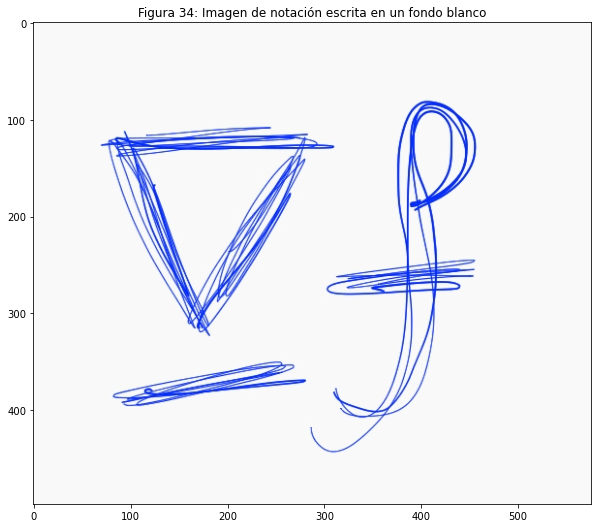
\includegraphics[width=\textwidth]{imagenes/PoissonImageEditing_cell_48_output_0.png}
        \caption{Imagen fuente}
    \end{subfigure}
     \begin{subfigure}[b]{.4\textwidth}
        \centering
        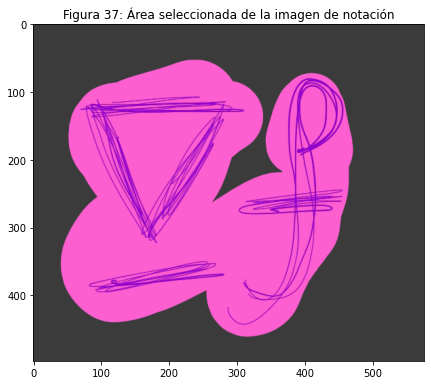
\includegraphics[width=\textwidth]{imagenes/PoissonImageEditing_cell_48_output_3.png}
        \caption{Región seleccionada}
    \end{subfigure}
    \begin{subfigure}[b]{.5\textwidth}
        \centering
        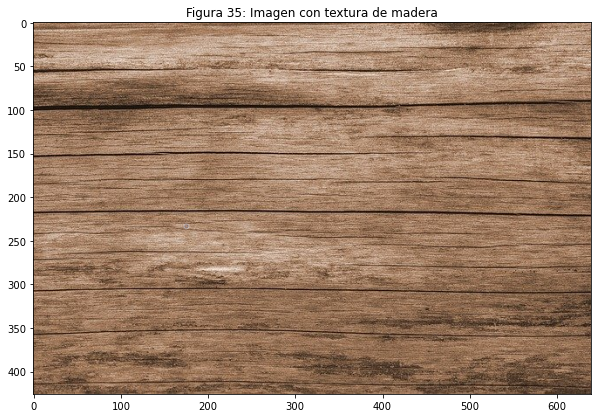
\includegraphics[width=\textwidth]{imagenes/PoissonImageEditing_cell_48_output_1.png}
        \caption{Imagen objetivo}
    \end{subfigure}
    \caption{Imágenes a usar en el ejemplo de inserción de objetos con agujeros}
    \label{fig:imagenesUsadasInsercionAgujeros}
\end{figure}

Tal y como se puede ver, la imagen fuente es una imagen de notación (similar a la del artículo) con agujeros. La imagen destino será una pared de madera.

\begin{figure}[h]
    \centering
    \begin{subfigure}[b]{.5\textwidth}
        \centering
        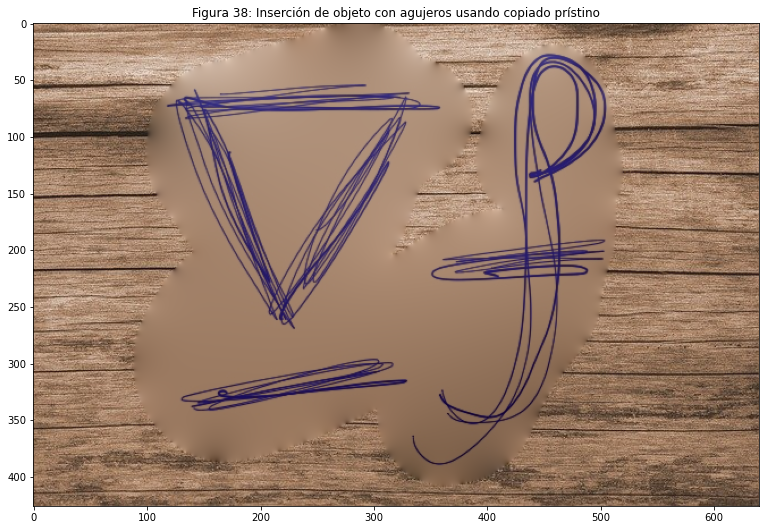
\includegraphics[width=\textwidth]{imagenes/PoissonImageEditing_cell_50_output_0.png}
        \caption{Resultado usando copiado prístino}
        \label{fig:resultadoAgujerosCopiadoPristino}
    \end{subfigure}%
    \begin{subfigure}[b]{.5\textwidth}
        \centering
        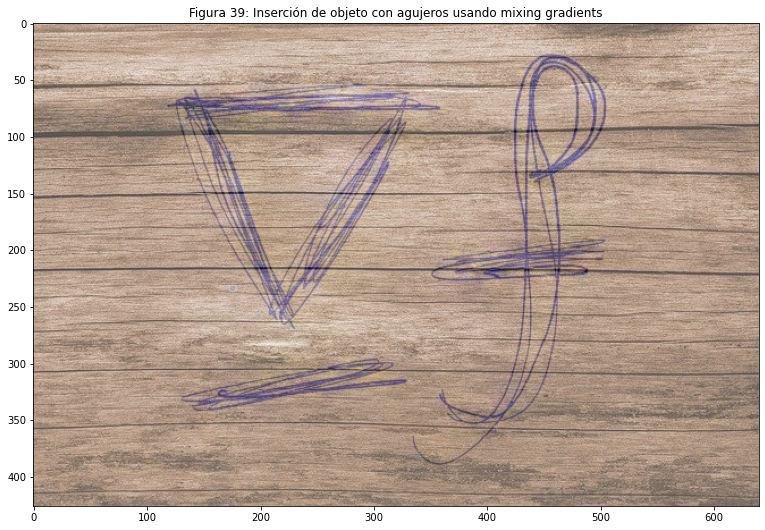
\includegraphics[width=\textwidth]{imagenes/PoissonImageEditing_cell_50_output_1.png}
        \caption{Resultado usando mezcla de gradientes}
        \label{fig:resultadoAgujerosMixingGradients}
    \end{subfigure}
    \caption{Resultados obtenidos insertando un objeto con agujeros}
    \label{fig:resultadosInsercionAgujeros}
\end{figure}

En \textit{Figura \ref{fig:resultadosInsercionAgujeros}} se pueden observar los resultados obtenidos usando las dos técnicas presentadas. En \textit{Figura \ref{fig:resultadoAgujerosCopiadoPristino}} es posible comprobar que, usando copiado prístino, la información de la textura de la madera en los agujeros es eliminada completamente. Sin embargo, en \textit{Figura \ref{fig:resultadoAgujerosMixingGradients}}, , usando la técnica de \textbf{mezcla de gradientes}, la información de la textura de la madera es conservada en la inserción, consiguiendo un resultado mucho más realista y esperado.

\subsection{Inserción de objetos transparentes}
\label{subsection:InsercionObjetosTransparente}
En la figura \ref{fig:arcoirisCopiadoPristino} se ha podido comprobar el resultado de la inserción de un objeto transparente (un arcoíris) sobre una imagen destino. No obstante, dicho resultado no era del todo realista ya que mucha información de la playa se perdía. A continuación reproduciremos el mismo ejemplo pero, en este caso, usando la técnica de \textbf{mezcla de gradientes}. La celda de código correspondiente a la recreación de este caso es \texttt{Código 22}.

\begin{figure}[h]
    \centering
    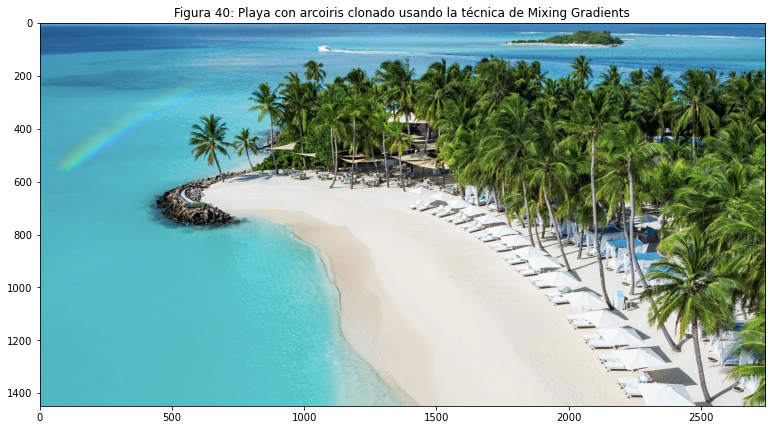
\includegraphics[width=.7\textwidth]{imagenes/PoissonImageEditing_cell_53_output_0.png}
    \caption{Resultados obtenidos insertando un objeto transparente}
    \label{fig:resultadosObjetoTransparente}
\end{figure}

En \textit{Figura \ref{fig:resultadosObjetoTransparente}} es posible observar que con la técnica de \textbf{mezcla de gradientes} se ha conseguido un resultado más realista. En particular, mientras que en la figura \ref{fig:arcoirisCopiadoPristino} además de perderse cierta información en la zona del agua, también se ha introducida una pequeña distorsión cerca del área de una de las palmeras. Sin embargo, en el último resultado obtenido esto no sucede, conduciendo a un resultado más esperado y realista, lo cual era lo que se pretendía.

\subsection{Inserción de un objeto cerca de otro}

Otro caso en el que es útil la aplicación de la técnica de \textbf{mezcla de gradientes} es cuando se desea realizar la inserción de un objeto de la imagen fuente cerca de otro objeto en la imagen destino. Tal y como se ha podido comprobar en ejemplos anteriores, cuando esta situación se produce, la técnica de copiado prístino crea distorsiones en la frontera de ambos objetos. Este aspecto es el que se quiere solucionar con la técnica presentada en esta sección. En \textit{Figura \ref{fig:imagenesUsadasInsercionCerca}} se pueden observar las imágenes consideradas para la aplicación de este caso. Las celdas de código correspondientes a la recreación de este caso son \texttt{Código 23} y \texttt{Código 24}.

\begin{figure}[h]
    \centering
    \begin{subfigure}[t]{.45\textwidth}
        \centering
        \includegraphics[width=\textwidth]{imagenes/PoissonImageEditing_cell_56_output_0.png}
        \caption{Imagen fuente}
    \end{subfigure}
    \begin{subfigure}[t]{.45\textwidth}
        \centering
        \includegraphics[width=\textwidth]{imagenes/PoissonImageEditing_cell_56_output_3.png}
        \caption{Región seleccionada a insertar}
    \end{subfigure}
    \begin{subfigure}[t]{.45\textwidth}
        \centering
        \includegraphics[width=\textwidth]{imagenes/PoissonImageEditing_cell_56_output_1.png}
        \caption{Imagen objetivo}
    \end{subfigure}
    \caption{Imágenes a usar en el ejemplo de inserción de objetos con agujeros}
    \label{fig:imagenesUsadasInsercionCerca}
\end{figure}

% Figuras avionetas por el desierto  por copiado prístino y mezclado gradientes 

\begin{figure}[h]
    \centering
    \begin{subfigure}[b]{.45\textwidth}
        \centering
        \includegraphics[width=\textwidth]{imagenes/PoissonImageEditing_cell_58_output_0.png}
        \caption{Resultado usando copiado prístino}
        \label{fig:resultadoInsercionCercaCopiadoPristino}
    \end{subfigure}%
    \begin{subfigure}[b]{.45\textwidth}
        \centering
        \includegraphics[width=\textwidth]{imagenes/PoissonImageEditing_cell_58_output_1.png}
        \caption{Resultado usando mezcla de gradientes}
        \label{fig:resultadoInsercionCercaMixingGradients}
    \end{subfigure}
    \caption{Resultados obtenidos insertando un objeto cerca de otro}
    \label{fig:resultadosInsercionCerca}
\end{figure}

En \textit{Figura \ref{fig:resultadosInsercionCerca}} se puede visualizar las diferencias entre copiado prístino y mezcla de gradientes para el caso tratado. Mientras que en \textit{Figura \ref{fig:resultadoInsercionCercaCopiadoPristino}} se producen distorsiones cerca del borde de la duna de arena, en \textit{Figura \ref{fig:resultadoInsercionCercaMixingGradients}} se puede comprobar que dichas distorsiones desaparecen, conduciendo a un resultado mucho más deseado y realista, lo cual era lo que se pretendía.

\subsection{Conclusiones}

Tras la experimentación con todos los ejemplos anteriormente presentados, podemos concluir que la técnica \textbf{mezcla de gradientes} es bastante útil, además de obtener buenos resultados.

A la vista de las mejoras producidas frente a la técnica de copiado prístino (\ref{tecnica:copiadoPristino}) no debe caerse en el error de lo anecdótico y pensar que la técnica de gradiente (\ref{tecnica:mezcladoDeGradiente}) es una mejora general del primero.  Tengamos claro que es un refinamiento para casos particulares en los que por la naturaleza topológica o transparencia de la región a copiar es conveniente utilizar la técnica de mezclado para considerar la imagen fuente y destino.  

Una ventaja que permite la técnica de mezclado es una selección relajada del área que se desea insertar, notemos cómo en la   figura \label{fig:imagenesUsadasInsercionCerca} la región seleccionada dista bastante de captar solo el humo y el avión; o incluso un caso más radical, en la figura \label{fig:imagenesUsadasInsercionAgujeros}, hubiera sido muy complejo la inserción trazo por trazo de la imagen. seleccionar trazo por trazo. 

En definitiva, la principal razón detrás de elegir una técnica u otra está en si desea considerar la información de la imagen destino, $f^*$, en la región a insertar, $\Omega$. Así mismo, hay que destacar que la técnica de mezcla de gradientes sólo es un caso particular de definir el vector guía de campo, $v$, como una combinación no lineal usando los gradientes de ambas imágenes. Según el resultado que se desee obtener, se puede definir otra combinación no lineal, dando lugar al desarrollo de una nueva técnica.

\newpage

\section{Técnica de aplanado de texturas}

\subsection{Fundamento y descripción}

Con esta técnica lo que se pretende es aplanar las texturas de una imagen. Aclarar que, dado que el objetivo de esta técnica es la alteración de una imagen, se considera la imagen destino como una copia de la imagen fuente, es decir, $f^* = g$. La idea que subyace detrás de esta técnica es la siguiente: si se desean aplanar texturas será necesario eliminar cambios de color, frecuencias, no representativos. No obstante, es necesario mantener aquellos que dotan de identidad a la imagen. Para conseguir dicho objetivo se definirá el vector guía de campo a partir del gradiente de la imagen, $\nabla f^*$, a través de un detector para detener las características más relevantes de una imagen. De este modo, la definición del vector guía de campo es:

\begin{equation}
    \forall x \in \Omega, v(x) = M(x) \nabla f^*(x)
\end{equation}

Donde $M$ es una máscara binaria, con activación en puntos de interés de la imagen. En el propio artículo \cite{poissonImageEditing} se indica que una buena elección para dicha máscara binaria podría ser un detector de bordes.

La versión discreta de la definición del vector guía de campo anteriormente comentado es:

\begin{equation}
    v_{pq}=\left\{
                \begin{array}{ll}
                  f_p^* - f_q^*, & \text{si hay un borde entre $p$ y $q$}\\
                  0, & \text{en caso contrario}\\
                \end{array}
          \right.
\end{equation}

La implementación de dicha definición se encuentra en la celda \texttt{Código 25} del código notebook.

Como prueba inicial, usamos como máscara binaria los puntos de interés detectados por el algoritmo SIFT. Sin embargo, los resultados fueron malos. Esto se debe a que la cantidad de puntos extraídos mediante SIFT no eran los suficientes como para obtener un efecto notorio en la imagen. Lo que pone de manifiesto la importancia que tiene en esta técnica el detector usado:

\begin{itemize}
    \item Si el detector usado extrae pocos puntos de interés, la calidad del resultado final será mala debido a que se aplanará casi toda la región.
    \item Si el detector usado extrae demasiados puntos de interés, la aplicación de esta técnica tendrá poco o nulo impacto en el resultado final (sólo se aplanarán pocas áreas de las imágenes).
\end{itemize}

La conclusión que se extrae es que hay obtener un equilibrio en los puntos extraídos por el detector, considerando las características de la imagen que se está tratando y haciendo un ajuste de los parámetros del detector (si los tiene) para dicha imagen concreta.

\begin{figure}[h]
    \centering
    \includegraphics[width=.5\textwidth]{imagenes/PoissonImageEditing_cell_66_output_0.png}
    \caption{Imagen que va ser usada en la técnica de aplanado de texturas}
    \label{fig:imagenAplanadoTexturas}
\end{figure}

En \textit{Figura \ref{fig:imagenAplanadoTexturas}} se presenta la imagen con la que se va a reproducir un ejemplo para esta técnica, la imagen del rostro de una niña.

\subsection{Elección de un detector de bordes}

Una forma de detectar bordes vista en teoría es la de convolucionar la imagen con un filtro de derivada gaussiana: aquellos píxeles con valores distintos de 0 pueden ser considerados como bordes. Sin embargo, esta técnica tiene un problema y es que es altamente sensible al ruido. Es por ello por lo que decidimos usar algún detector de bordes que presentase mayor robustez que la técnica vista en teoría.

Leyendo la documentación presente en `OpenCV` \cite{canyOpenCV} encontramos un detector de bordes que, a priori, parecía obtener buenos resultados: \textit{Canny Edge Detection}. Dicho algoritmo opera en los siguiente pasos:

\begin{enumerate}
    \item \textbf{Reducción de ruido}. Debido a que la detección de bordes es susceptible al ruido en la imagen, lo primero que se realiza es convolucionar la imagen con un filtro gaussiano de dimensiones $5x5$. Como se ha visto en teoría, esta aproximación es bastante común a la hora de intentar reducir el ruido presente en una imagen.
    \item Se aplica un \textbf{filtro de Sobel} (en ambos ejes, $X$ e $Y$) para después computar la intensidad del gradiente en la imagen. La ventaja de esta aproximación reside en que se tienen en cuenta las derivadas de la imagen en ambos ejes (los bordes detectados no dependen del eje).
    \item A través de la información de la magnitud del gradiente y su dirección se realiza un barrido de toda la imagen para \textbf{detectar aquellos píxeles que son un máximo local} de su vecindario. El valor de los píxeles descartados en este paso es puesto a 0 (\textit{Non-Maximum Suppression}).
    \item Se aplica un \textbf{refinamiento de los píxeles} encontrados en el paso anterior a partir de los parámetros dados al detector: los píxeles con valores mayor al ''umbral máximo'' son considerados como bordes fuertes, los píxeles con valores menor al ''umbral mínimo'' son descartados y para aquellos píxeles con valores entre ambos umbrales se realiza una evaluación dependiendo de su conectividad a los bordes fuertes.
\end{enumerate}

Debido a que la metodología seguida por el detector nos pareció más que razonable, y además, teniendo en cuenta que dicho de detector ya viene implementado en la biblioteca \textit{OpenCV}, nos dispusimos a hacer pruebas. Dichas pruebas se encuentran en la celda \texttt{Código 28} del código notebook.

En la celda \texttt{Código 27} se encuentra la implementación de la función \textit{CannyEdgeDetection}, función que computa los bordes en la imagen haciendo uso del algoritmo \textit{Canny} de la biblioteca \textit{OpenCV}. Dicha función acepta los siguientes parámetros:

\begin{itemize}
    \item \textit{img}: Imagen de la que se desea extraer los bordes.
    \item \textit{sobelSize}: Tamaño del filtro de Sobel que se quiere usar para derivar la imagen.
    \item \textit{minVal}: Valor mínimo para que un píxel no sea descartado.
    \item \textit{maxVal}: Valor mínimo para que un píxel sea considerado un borde seguro.
\end{itemize}

También hay que aclarar que el parámetro \textit{L2gradient} del detector Canny presente en \textit{OpenCV} será establecido a \textit{False} en todas nuestras pruebas (Se usará la norma $L_1 = 
|dI/dx| + |dI/dy|$). Esta decisión se fundamenta en que, si bien la norma $L_2$ puede proporcionar mayor precisión, el gasto en tiempo computacional no lo compensa.

\subsection{Experimentación con el detector de bordes}

El siguiente paso en la reproducción del ejemplo para la técnica de aplanado de texturas es determinar los parámetros óptimos del detector de bordes para la imagen elegida.

\begin{figure}[h]
    \centering
    \begin{subfigure}[b]{.3\textwidth}
        \centering
        \includegraphics[width=\textwidth]{imagenes/PoissonImageEditing_cell_70_output_0.png}
        \caption{Primera aproximación}
        \label{fig:1Aprox}
    \end{subfigure}%
    \centering
    \begin{subfigure}[b]{.3\textwidth}
        \centering
        \includegraphics[width=\textwidth]{imagenes/PoissonImageEditing_cell_70_output_1.png}
        \caption{Segunda aproximación}
        \label{fig:2Aprox}
    \end{subfigure}%
    \centering
    \begin{subfigure}[b]{.3\textwidth}
        \centering
        \includegraphics[width=\textwidth]{imagenes/PoissonImageEditing_cell_70_output_2.png}
        \caption{Tercera aproximación}
        \label{fig:3Aprox}
    \end{subfigure}
    \centering
    \begin{subfigure}[b]{.3\textwidth}
        \centering
        \includegraphics[width=\textwidth]{imagenes/PoissonImageEditing_cell_70_output_3.png}
        \caption{Cuarta aproximación}
        \label{fig:4Aprox}
    \end{subfigure}%
    \centering
    \begin{subfigure}[b]{.3\textwidth}
        \centering
        \includegraphics[width=\textwidth]{imagenes/PoissonImageEditing_cell_70_output_4.png}
        \caption{Quinta aproximación}
        \label{fig:5Aprox}
    \end{subfigure}%
    \centering
    \begin{subfigure}[b]{.3\textwidth}
        \centering
        \includegraphics[width=\textwidth]{imagenes/PoissonImageEditing_cell_70_output_5.png}
        \caption{Sexta aproximación}
        \label{fig:6Aprox}
    \end{subfigure}
    \caption{Bordes detectados variando parámetros del detector de bordes}
    \label{fig:bordesCanny}
\end{figure}

Como es posible observar en \textit{Figura \ref{fig:bordesCanny}}, para la \textit{Figura \ref{fig:1Aprox}} y para la \textit{Figura \ref{fig:2Aprox}} los resultados, en el caso de esta imagen, no son buenos, bien porque los parámetros usados han conducido a que el algoritmo sea muy sensible o bien porque han conducido a que el algoritmo sea poco sensible. Sin embargo, para la \textit{Figura \ref{fig:3Aprox}}, el resultado, a nivel visual, es correcto. Un refinamiento se puede encontrar en \textit{Figura \ref{fig:4Aprox}}, figura para la que se ha encontrado el mejor resultado.

Posteriormente, en \textit{Figura \ref{fig:5Aprox}} y en \textit{Figura \ref{fig:6Aprox}} se han realizado más pruebas variando la apertura del filtro de Sobel. Sin embargo, para dichas pruebas se han hallado resultados similares. Por simplicidad y eficiencia se tomará la \textit{Figura \ref{fig:4Aprox}} para el cómputo del aplanado de texturas como máscara binaria, es decir, $M$.

\subsection{Resultado final}

\begin{figure}[h]
    \centering
    \includegraphics[width=.5\textwidth]{imagenes/PoissonImageEditing_cell_73_output_0.png}
    \caption{Resultado final de la técnica de aplanado de texturas}
    \label{fig:resultadoAplanadoTexturas}
\end{figure}

En la \textit{Figura \ref{fig:resultadoAplanadoTexturas}} se puede apreciar el resultado final de la aplicación de esta técnica. Es fácil ver cómo la información de las características más importantes del rostro (ojos, cejas, nariz y boca) son mantenidas (sufriendo un pequeño aplanamiento, lo cual es totalmente esperable); mientras que la información de las demás características es aplanada, lo cual era lo que se pretendía con el uso de esta técnica.

\subsection{Conclusiones}

Como se ha podido comprobar, con esta técnica es posible obtener buenos resultados, sin embargo, presenta algunos inconvenientes:

\begin{itemize}
    \item \textbf{Elección del detector a usar}: Es necesario definir qué detector de puntos de interés se va a usar. La elección del detector también puede llegar a afectar a la definición del vector guía de campo, reduciendo la automatización del proceso (sería necesaria la revisión/implementación del vector guía de campo por un humano).
    \item \textbf{Hay que tener en cuenta las características del detector usado}: Como anteriormente se ha comentado, el número de puntos extraídos por el detector puede llegar a afectar negativamente al resultado final. Por ello es necesario la experimentación/comprobación de este aspecto, reduciendo otra vez la automatización del proceso.
    \item \textbf{Hay que tener en cuenta las características de la imagen}: No todas las imágenes poseen las mismas características, puede haber cambios de luminosidad, cambios de perspectiva,... Es por ello por lo que hay que hacer un ajuste de los parámetros usados por el detector para cada caso particular, lo cual supone otro aspecto que reduce la automatización.
\end{itemize}

En definitiva, encontramos el uso de esta técnica bastante interesante puesto que con ella se obtienen buenos resultados, siempre que se escojan los parámetros adecuados. Hay que tener en cuenta que los resultados obtenidos mediante esta técnica dependen fuertemente de la máscara binaria considerada, por lo que a futuros, puede ser interesante experimentar con otras máscaras binarias.

\newpage

\section{Técnica de cambios de iluminación locales}

\begin{figure}[h]
    \centering
    \begin{subfigure}[b]{.35\textwidth}
        \centering
        \includegraphics[width=\textwidth, height=5cm]{imagenes/PoissonImageEditing_cell_101_output_0.png}
        \caption{Naranja con brillo especular}
        \label{fig:naranjaBrillo}
    \end{subfigure}%
    \begin{subfigure}[b]{.3\textwidth}
        \centering
        \includegraphics[width=\textwidth, height=5cm]{imagenes/PoissonImageEditing_cell_101_output_2.png}
        \caption{Hombre subexpuesto}
        \label{fig:hombreOscuro}
    \end{subfigure}
    \caption{Imágenes de ejemplo para la técnica de cambios de iluminación locales}
    \label{fig:ejemplosCambiosIluminación}
\end{figure}

\subsection{Fundamento y descripción}

El propósito de esta técnica es la de realizar cambios locales en la iluminación de una imagen, como por ejemplo añadir luminosidad a una región o la eliminación de reflejos especulares.

Tal y como se indica en el artículo \cite{poissonImageEditing}, siguiendo el trabajo del método establecido en \cite{fattal_lischinski_werman_2002} (en el cual se usa el vector $v$ para reconstruir el logaritmo de la imagen, $f$, mediante la resolución de la ecuación de Poisson $\nabla f = div(\boldsymbol{v})$ en el dominio de la imagen usando condiciones de contorno de Neumann), una extensión natural es restringir la corrección a una región $\Omega$ usando condiciones apropiadas de Dirichlet en $\partial\Omega$. De esta manera, usando una versión simplificada de la transformación del artículo anterior, el vector de guía de campo es definido en el dominio logarítmico de la siguiente manera:

\begin{equation}
    \boldsymbol{v} = \alpha^{\beta}|\nabla f^*|^{-\beta}\nabla f^*
\end{equation}

Con $\alpha = 0.2$ veces el promedio de la norma del gradiente de $f^*$ sobre $\Omega$ y $\beta=0.2$.

Las funciones implementadas para la aplicación de esta técnica se encuentran disponibles en la celda \texttt{Código 40} del código notebook. La primera de ellas es \textit{MagnitudeGradient}, función que computa la magnitud del gradiente de una imagen. Dicho cálculo se realiza de la misma manera que se ha explicado en teoría y prácticas:

\begin{enumerate}
    \item Se computa una máscara gaussiana y una máscara derivativa. En este caso se van a tomar máscaras binomiales para el alisamiento y máscaras de Sobel para el cómputo de la derivada de la imagen. Esta decisión ha sido en base a que \textit{OpenCV} ofrece, sin afectar a los resultados, una función con una interfaz muy cómoda para el cálculo de las derivadas de una imagen: \textit{cv.Sobel()}.
    \item Dependiendo del eje en el que se desee calcular la derivada, la convolución se realiza alisando a través de un eje (aplicando la máscara binomial) y convolucionando con la máscara de Sobel en el otro eje. El resultado es la derivada de la imagen en ese eje, tal y como se ha visto en teoría.
    \item La magnitud del gradiente se obtiene como: $|\nabla I| = \sqrt{(\frac{\partial I}{\partial x})^2 + (\frac{\partial I}{\partial y})^2}$ siendo $I$ la imagen de la que se desea computar la magnitud del gradiente.
\end{enumerate}

La otra función implementada fue \textit{LocalIlluminationVector}, función que define el vector guía de campo necesario para la aplicación de esta técnica, acorde a la ecuación anteriormente mencionada.

\subsection{Ejemplos}

En la \textit{Figura \ref{fig:ejemplosCambiosIluminación}} se pueden observar las imágenes con las que se va a tratar en la aplicación de esta técnica. \textit{Figura \ref{fig:naranjaBrillo}} representa un caso de eliminación de brillo especular mientras que \textit{Figura \ref{fig:hombreOscuro}} representa un caso de alzamiento de iluminación.

Cabe aclarar que se realizará una batería de pruebas para varios valores de $\alpha$ y $\beta$.

\begin{figure}[h]
    \centering
    \begin{subfigure}[b]{.43\textwidth}
        \centering
        \includegraphics[width=\textwidth]{imagenes/PoissonImageEditing_cell_103_output_0.png}
        \caption{Primera aproximación}
        \label{fig:Naranja1Aprox}
    \end{subfigure}%
    \centering
    \begin{subfigure}[b]{.47\textwidth}
        \centering
        \includegraphics[width=\textwidth]{imagenes/PoissonImageEditing_cell_103_output_1.png}
        \caption{Segunda aproximación}
        \label{fig:Naranja2Aprox}%
    \end{subfigure}
    \centering
    \begin{subfigure}[b]{.45\textwidth}
        \centering
        \includegraphics[width=\textwidth]{imagenes/PoissonImageEditing_cell_103_output_2.png}
        \caption{Tercera aproximación}
        \label{fig:Naranja3Aprox}
    \end{subfigure}%
    \centering
    \begin{subfigure}[b]{.45\textwidth}
        \centering
        \includegraphics[width=\textwidth]{imagenes/PoissonImageEditing_cell_103_output_3.png}
        \caption{Cuarta aproximación}
        \label{fig:Naranja4Aprox}%
    \end{subfigure}
    \caption{Resultados obtenidos intentando eliminar el brillo especular de la naranja}
    \label{fig:resultadosNaranja}
\end{figure}

En la \textit{Figura \ref{fig:resultadosNaranja}} se pueden observar los resultados obtenidos para los sucesivos valores comentados anteriormente. Se puede apreciar cómo hay un refinamiento sucesivo del resultado, llegando a un resultado excelente en \textit{Figura \ref{fig:Naranja4Aprox}}, resultado en el que se ha conseguido eliminar casi por completo el brillo especular de la naranja. Dicho resultado ha sido conseguido con la combinación de valores $\alpha = 0.05$ y $\beta = 0.4$.

\begin{figure}[h]
    \centering
    \begin{subfigure}[b]{.44\textwidth}
        \centering
        \includegraphics[width=\textwidth]{imagenes/PoissonImageEditing_cell_103_output_4.png}
        \caption{Primera aproximación}
        \label{fig:Hombre1Aprox}
    \end{subfigure}%
    \centering
    \begin{subfigure}[b]{.46\textwidth}
        \centering
        \includegraphics[width=\textwidth]{imagenes/PoissonImageEditing_cell_103_output_5.png}
        \caption{Segunda aproximación}
        \label{fig:Hombre2Aprox}%
    \end{subfigure}
    \centering
    \begin{subfigure}[b]{.45\textwidth}
        \centering
        \includegraphics[width=\textwidth]{imagenes/PoissonImageEditing_cell_103_output_6.png}
        \caption{Tercera aproximación}
        \label{fig:Hombre3Aprox}
    \end{subfigure}%
    \centering
    \begin{subfigure}[b]{.45\textwidth}
        \centering
        \includegraphics[width=\textwidth]{imagenes/PoissonImageEditing_cell_103_output_7.png}
        \caption{Cuarta aproximación}
        \label{fig:Hombre4Aprox}%
    \end{subfigure}
    \caption{Resultados obtenidos intentando alzar la iluminación en la región del hombre subexpuesto}
    \label{fig:resultadosHombre}
\end{figure}

En la \textit{Figura \ref{fig:resultadosHombre}} pueden observarse los distintos resultados obtenidos para la combinación de valores anteriormente comentada. Es curioso observar como, al contrario de lo que pasaba en el caso de la naranja, hay un sucesivo empeoramiento de los resultados. De este modo, el mejor resultado ha sido obtenido en la \textit{Figura \ref{fig:Hombre1Aprox}}, figura en la que se ha producido un alzamiento realista de la región ocupada por el hombre, no como en los demás resultados, donde el alzado ha sido tan brusco que hasta llega a ser poco creíble. Dicho resultado ha sido conseguido con la combinación de valores $\alpha = \beta = 0.2$.

\subsection{Conclusiones}

Tras la experimentación realizada con esta técnica hemos encontrado las siguientes limitaciones en la misma:

\begin{itemize}
    \item \textbf{La selección de la región debe de ser precisa}: Esto es debido a que si la región es demasiado amplia, probablemente se esté considerando información no deseada en el cálculo del promedio de la norma del gradiente, conduciendo a resultados incorrectos.
    \item \textbf{Se ha de realizar un refinamiento de los parámetros usados}: Tal y como se ha podido comprobar en la experimentación anterior, los valores de $\alpha$ y $\beta$ dependen altamente de la imagen a tratar. Es necesario un refinamiento manual seleccionando aquellos parámetros con los que se consiguen los mejores resultados.
\end{itemize}

En definitiva, encontramos el uso de esta técnica bastante interesante puesto que con ella se consiguen resultados muy buenos (desde la perspectiva visual). Sin embargo, las limitaciones anteriormente comentadas reducen la automatización del proceso puesto que es necesaria la interacción del usuario para el refinamiento de los parámetros.

\newpage

\section{Técnica de cambios locales de color}

\subsection{Fundamento y descripción}

El propósito de esta técnica es la manipulación de los colores de una imagen en una región seleccionada, $\Omega$, todo ello mediante la aplicación de la ecuación de Poisson.

El uso de esta técnica tiene un interés múltiple:

\begin{itemize}
    \item El \textbf{problema de decolorear} la imagen a excepción de una región de interés ha sido tratado manualmente mediante la selección manual exacta de dicha región. Sin embargo, la edición de imágenes a través de la ecuación de Poisson libera al usuario de dicha selección "perfecta". En este caso la imagen destino, $f^*$, se establece como la luminancia de la imagen fuente, $g$. Una vez realizada dicha conversión, la selección del objeto se puede realizar \textbf{relajando la precisión}. Finalmente el resultado se obtiene resolviendo la ecuación de Poisson para cada canal. Cabe mencionar que, debido a la dificultad del cálculo de la luminancia en el caso de una imagen, se tomará la versión en escala de grises como sustituto.
    \item También puede usarse para \textbf{alterar el color} del objeto en cuestión. En este caso, antes de resolver la ecuación de Poisson, la imagen fuente es copiada y considerada como $f^*$. Una versión con colores modificados es considerada la imagen fuente, es decir, $g$.
\end{itemize}

Para una imagen a color y una región de ella $\Omega$ coloreada de dos versiones $v_1$, $v_2$  (de forma diferente) pueden ser mezcladas usando el copiado prístino: una versión cualquiera $v_1$ se usa como imagen destino, es decir, $f^*$ fuera de $\Omega$ y la otra versión $v_2$, se usa como imagen fuente, la función $g$ a ser modificada dentro de $\Omega$. 

Notése que para la aplicación de dicha técnica no es necesario la implementación de ninguna función. Lo que sí se debe de hacer es formar correctamente las imágenes destino y fuente de la misma manera en la que se comenta en el artículo \cite{poissonImageEditing}. Comentar también que el caso que se va a replicar para la experimentación con estas técnicas será similar al del presentado en el artículo: una flor amarilla sobre un fondo verde. En la celda \texttt{Código 43} se realiza la lectura de la imagen y el cómputo de la región, $\Omega$.

\begin{figure}[h]
    \centering
    \begin{subfigure}[t]{.45\textwidth}
        \centering
        \includegraphics[width=\textwidth]{imagenes/PoissonImageEditing_cell_107_output_0.png}
        \caption{Imagen de flor amarilla sobre la que se van a realizar cambios de colores}
        \label{fig:florAmarilla}
    \end{subfigure}%
    \centering
    \begin{subfigure}[t]{.45\textwidth}
        \centering
        \includegraphics[width=\textwidth]{imagenes/PoissonImageEditing_cell_107_output_2.png}
        \caption{Región seleccionada de la flor amarilla}
        \label{fig:regionFlorAmarilla}%
    \end{subfigure}
    \caption{Imagen y región a tratar en la aplicación de los cambios locales de color}
    \label{fig:ejemploCambiosColoLocales}
\end{figure}

En \textit{Figura \ref{fig:florAmarilla}} es posible observar la imagen con la que se va a tratar en la aplicación de esta técnica y en \textit{Figura \ref{fig:regionFlorAmarilla}} la selección de la región, que, como puede observarse, no es precisa.

\subsection{Resultados}

El primer caso presentado será la decolorización del fondo de la imagen (a excepción del objeto de interés). Dicho caso se puede encontrar en la celda \texttt{Código 44} del código notebook.

\begin{figure}[h]
    \centering
    \begin{subfigure}[t]{.45\textwidth}
        \centering
        \includegraphics[width=\textwidth]{imagenes/PoissonImageEditing_cell_109_output_0.png}
        \caption{Imagen en escala de grises}
        \label{fig:florGrises}
    \end{subfigure}%
    \centering
    \begin{subfigure}[t]{.45\textwidth}
        \centering
        \includegraphics[width=\textwidth]{imagenes/PoissonImageEditing_cell_109_output_1.png}
        \caption{Decoloración del fondo de la imagen}
        \label{fig:resultadoDecolorizacion}%
    \end{subfigure}
    \caption{Resultados obtenidos para el caso de decolorización de la imagen}
    \label{fig:grisesResultadoDecolorizacion}
\end{figure}

La \textit{Figura \ref{fig:florGrises}} es la versión en escala de grises de la imagen multibanda (se triplica en los 3 canales la escala de grises monobanda). La \textit{Figura \ref{fig:resultadoDecolorizacion}} es el resultado final obtenido para este caso. Es preciso comentar, que aunque el resultado parece ofrecer una segmentación del objeto de interés, este no es  realmente el caso debido a que hay pequeñas distorsiones alrededor de la región seleccionada.

A continuación se va a realizar la aplicación del segundo caso anteriormente comentado, el cambio de color. Para ello, se multiplican los canales BGR de la imagen original por 0.5, 0.5 y 1.5 respectivamente para formar la imagen fuente. La implementación de este caso se encuentra en la celda \texttt{Código 45} del código notebook.

\begin{figure}[h]
    \centering
    \includegraphics[width=.5\textwidth]{imagenes/PoissonImageEditing_cell_111_output_0.png}
    \caption{Resultado final de cambio de color en el objeto de interés con tonos rojos}
    \label{fig:resultadoFlorRoja}
\end{figure}

Tal y como se puede observar en \textit{Figura \ref{fig:resultadoFlorRoja}}, el resultado es bastante correcto a nivel visual, tornándose el color de la flor de amarillo a un tono anaranjado. Como es lógico pensar, ¿qué ocurre si se potencia otra banda de la imagen en lugar de la banda roja? Hicimos pruebas para ver lo que ocurría, intercambiando los factores multiplicativos anteriormente mencionados. Dichas pruebas se encuentran en la celda \texttt{Código 46.a} del código notebook.

\begin{figure}[h]
    \centering
    \begin{subfigure}[t]{.45\textwidth}
        \centering
        \includegraphics[width=\textwidth]{imagenes/PoissonImageEditing_cell_113_output_0.png}
        \caption{Resultado potenciando la banda verde}
        \label{fig:bandaVerdeFlor}
    \end{subfigure}
    \centering
    \begin{subfigure}[t]{.45\textwidth}
        \centering
        \includegraphics[width=\textwidth]{imagenes/PoissonImageEditing_cell_113_output_1.png}
        \caption{Resultado potenciando la banda azul}
        \label{fig:bandaAzulFlorIni}%
    \end{subfigure}
    \caption{Resultados obtenidos potenciando diversas bandas de la imagen multicanal}
    \label{fig:resultadosPotenciacionBandas}
\end{figure}

Como se puede observar en \textit{Figura \ref{fig:bandaVerdeFlor}}, el resultado obtenido dándole más importancia al canal verde de la imagen es bastante bueno a nivel visual, ya que cambiar el color de los pétalos y al estar sobre fondo verde no se aprecia la distorsión.

Sin embargo, en \textit{Figura \ref{fig:bandaAzulFlorIni}} al intentar relajar al canal azul de la imagen el resultado no se obtiene un cambio de color sino de la intensidad general, volviéndonos con ello a encontrar una flor amarilla.  Esto se debe el color amarillo estándar en RGB es [255, 233, 0]. 
Es decir, la información aportada por el canal azul para la región seleccionada de la flor es mínima.    

Esto podría plantear que el método tuviera una limitación en cuanto a la obtención de toda la gama colores.

\subsection{Técnica de intercambio de color modificada}

La limitación del método propuesto en \cite{poissonImageEditing} reside en que un canal de la región seleccionada tenga valores por lo general próximos a cero(por ejemplo canal azul \textit{Figura \ref{fig:bandaAzulFlorIni}}). La versión modificada de esta técnica se encuentra en la celda \texttt{Código 46.b} del código notebook.

\begin{figure}[h]
    \centering
    \begin{subfigure}[t]{.45\textwidth}
        \centering
        \includegraphics[width=\textwidth]{imagenes/PoissonImageEditing_cell_115_output_0.png}
        \caption{Imagen con los canales intercambiados}
        \label{fig:florCanalesIntercambiados}
    \end{subfigure}
    \centering
    \begin{subfigure}[t]{.45\textwidth}
        \centering
        \includegraphics[width=\textwidth]{imagenes/PoissonImageEditing_cell_115_output_1.png}
        \caption{Imagen con los canales intercambiados y ponderación aplicada}
        \label{fig:florCanalesPonderacion}%
    \end{subfigure}
    \caption{Resultados obtenidos potenciando diversas bandas de la imagen multicanal}
    \label{fig:resultadosPotenciacionBandas}
    \centering
    \begin{subfigure}[t]{.45\textwidth}
        \centering
        \includegraphics[width=\textwidth]{imagenes/PoissonImageEditing_cell_115_output_2.png}
        \caption{Resultado final potenciando la banda azul}
        \label{fig:bandaAzulFlorFin}%
    \end{subfigure}
    \caption{Resultados obtenidos mediante la nueva técnica de cambio de color}
    \label{fig:resultadosNuevaTecnicaCambiosColor}
\end{figure}

Por ello, para mantener \textit{la forma de la flor} pero conseguir que el canal azul aumente valores lo que hemos hecho es intercambiarlo por otro con valores mayores. Sin necesidad de comprobar numéricamente los canales, por ser los pétalos mayoritariamente amarillos, los canales rojo y verde tendrán valores mayores que el de azul. Por lo que  permutaremos los canales rojo y azul, obsérvese \textit{Figura \ref{fig:florCanalesIntercambiados}} de la imagen fuente. 

Tras esto se aplica el algoritmo de cambio de color obteniendo de manera exitosa el resultado buscado \textit{Figura \ref{fig:bandaAzulFlorFin}}. 

Observemos que el método es fácilmente generalizable, basta con tener conocimiento de los canales con mayores valores e intercambiarlos a conveniencia.

\subsection{Consideraciones sobre los factores multiplicativos de los canales}

En el artículo original \cite{poissonImageEditing}, no se da una cota de los valores que se pueden tomar y hasta ahora se han tomado de manera heurística y ajustado por prueba y error, partiendo de la base de que al multiplicar por un número mayor que uno potenciaremos un canal y por un valor entre 0 y 1 lo disminuiremos.   

Si se quisiera un procedimiento más matemático podría estudiarse la media $\mu$ de los distintos canales. 
Por tratarse de una imagen $0 \leq \mu \leq 255$ suponer que la distribución de la cantidad de píxeles que toman cierto valor sigue una distribución normal puede ser demasiado restrictivo.   

Luego como referencia que para cierto canal un coeficiente de $\frac{255}{\mu}$ saturará en media los píxeles del canal. Si se conociese la distribución se podría afinar el cálculo, por ejemplo si fuera una normal de desviación típica sabríamos exactamente el número de puntos.  

Sin duda para los ejemplo de esta práctica este coste es innecesario ya que por el método de inspección y prueba nos es suficiente, pero sin embargo, si la región fuera de una tamaño lo suficiente como para aumentar la demanda computacional, a partir de este tipo de heurísticas podría ahorrarse experimentaciones. 

\subsection{Conclusiones}

A la vista de los resultados hemos comprobado que el método efectivamente permite:

\begin{enumerate}
    \item Selección relajada de la región cromática en el problema de decoloreo. 
    \item Resultados relativamente exitosos en la recolorización de regiones.  
\end{enumerate}

El motivo por el cual (2) no es un rotundo éxito se debe a que si bien la selección sí puede hacerse de manera más relajada que en procedimiento totalmente manuales acaba introduciendo ruido y distorsiones fuera de la región objetivo (en nuestro caso particular el fondo tras la flor). Por otro lado la gama de colores a los que cambiar la región con el algoritmo del artículo \cite{poissonImageEditing} está condicionada a los valores de la imagen. Con nuestra propuesta se consigue mayor variabilidad, pero requiere de un esfuerzo adicional. 

\newpage

\section{Técnica de costura de imágenes}

\subsection{Fundamento y descripción}

Supóngase el caso en que dada una textura o una imagen se quiere ampliar su tamaño (sin realizar interpolación de píxeles) o crear un mosaico con ella. Una primera solución sería construir una imagen mayor por concatenación o repetición de la original, sin embargo, si la imagen no es idéntica en los bordes continuos en los que se \textit{pega} no es de extrañar que salgan resultados no deseables. 

En el artículo de referencia  \cite{poissonImageEditing} se  hace una propuesta en el caso de que el dominio de la imagen $\Omega$ sea rectangular, donde propone que adaptar los bordes de la imagen a repetir, formando una especie de costura que haga menos abrupto el pegado. 

Para ello fuerza ciertas condiciones periódicas en el contorno $\partial\Omega$ antes de computar la función de interpolación usando la ecuación de Poisson. En esta caso, la formulación del problema es la siguiente:

\begin{itemize}
    \item Denotaremos por $g$ a la imagen que se desea repetir, que en el caso de la ecuación de Poisson será la que veníamos detonando como \textit{imagen fuente}.
    \item Las condiciones de contorno se modifican de tal manera que lados opuestos del dominio rectangular se correspondan con condiciones idénticas de Dirichlet. Se puede establecer cualquier combinación lineal de los valores en el borde de la imagen, pero para casos genéricos entenderemos que todo los lados tiene la misma relevancia por lo que: 
    \begin{equation}
        f^*_{north} = f^*_{south} = 0.5 g_{north} + 0.5 g_{south} .
    \end{equation}
    \item De forma similar se computan las condiciones para el borde izquierdo y derecho de la imagen
\end{itemize}

La idea intuitiva de tomar la media de los valores del borde es para que los 4 bordes de la imagen resultado sean similares, de manera que la costura se pueda realizar en cualquier dirección (por arriba, por abajo, por la izquierda y por la derecha). Es decir, se le está dando la misma importancia a todos los bordes de las imágenes. Sin embargo, este aspecto es modificable según el resultado final que se desee (por ejemplo, se le puede dar más importancia al borde superior que al inferior).

El resultado de aplicar esta técnica es la obtención de una imagen con la que se puedan fabricar costuras mediante concatenación consecutiva.

Las implementaciones realizadas para la aplicación de esta técnica se encuentran en la celda \texttt{Código 35} del código notebook. La función \textit{SetRegionWithoutBorders} se encarga de obtener la región de píxeles de la imagen fuente eliminando los píxeles de los bordes. Esta selección de región es necesaria para que los valores se consideren adecuadamente. Luego la función \textit{TilingBoundaryConditions} se encarga de formar la imagen destino para la aplicación de esta técnica. Dicha imagen destino tendrá todos los valores de los píxeles establecidos a 0 a excepción de los píxeles de los bordes, los cuales tendrán los siguientes valores:

\begin{equation}
 f^*_{north} = f^*_{south} = \frac{g_{north} + g_{south}}{2}
\end{equation}

\begin{equation}
f^*_{east} = f^*_{west} = \frac{g_{east} + g_{west}}{2}
\end{equation}

\subsection{Resultados}

\begin{figure}[h]
    \centering
    \begin{subfigure}[t]{.3\textwidth}
        \centering
        \includegraphics[width=\textwidth]{imagenes/PoissonImageEditing_cell_89_output_0.png}
        \caption{Imagen original}
        \label{fig:costuraImgOriginal}
    \end{subfigure}
    \centering
    \begin{subfigure}[t]{.3\textwidth}
        \centering
        \includegraphics[width=\textwidth]{imagenes/PoissonImageEditing_cell_89_output_2.png}
        \caption{Imagen resultado}
        \label{fig:costuraResultado}
    \end{subfigure}
    \centering
    \begin{subfigure}[t]{.3\textwidth}
        \centering
        \includegraphics[width=\textwidth]{imagenes/PoissonImageEditing_cell_89_output_3.png}
        \caption{Diferencia de imágenes}
        \label{fig:costuraDiferencia}
    \end{subfigure}
    \caption{Resultados obtenidos mediante la aplicación de la técnica}
    \label{fig:resultadosCosturaImagenes}
\end{figure}

En \textit{Figura \ref{fig:costuraResultado}} es posible observar la imagen resultado. Si se realiza la comparación con la imagen original, \textit{Figura \ref{fig:costuraImgOriginal}}, es posible observar que la imagen resultado tiene un color más uniforme. Esto tiene sentido con la intención seguida por la técnica puesto que, si se desea realizar la costura de una imagen, el color de esta debe de ser uniforme (al menos en los bordes). Finalmente en \textit{Figura \ref{fig:costuraDiferencia}} se puede ver la diferencia entre la imagen original y la imagen resultado. La mayor diferencia se encuentra en los píxeles de los bordes (como era de esperar). Sin embargo, también se pueden ver diferencias en la parte superior y en la parte inferior de la imagen: esto casa con la aplicación de la técnica puesto que, si se observa la imagen original, la parte superior es más oscura que la inferior. Por ello la función de interpolación intenta corregir esta diferencia de intensidades mediante la modificación de los píxeles de dichas áreas (no ocurre lo mismo con las partes laterales de la imagen porque la intensidad es similar).

Una vez obtenido el resultado se puede proceder a realizar la costura mediante concatenación. La función que se encarga de realizar la costura se encuentra implementada en la celda \texttt{Código 37}: \textit{SewingImages}, función a la que se le pasa como parámetro una imagen y el número de costuras a realizar (tanto verticalmente como horizontalmente) y devuelve una imagen con la costura aplicada. Así mismo, en dicha celda se realiza las costuras de las imágenes de las celdas anteriores.

\begin{figure}[h]
    \centering
    \begin{subfigure}[t]{.3\textwidth}
        \centering
        \includegraphics[width=\textwidth]{imagenes/PoissonImageEditing_cell_91_output_0.png}
        \caption{Costura con la imagen original}
        \label{fig:costuraConcatOriginal}
    \end{subfigure}
    \centering
    \begin{subfigure}[t]{.3\textwidth}
        \centering
        \includegraphics[width=\textwidth]{imagenes/PoissonImageEditing_cell_91_output_1.png}
        \caption{Costura con la imagen resultado}
        \label{fig:costuraImgResultado}
    \end{subfigure}
    \caption{Resultados obtenidos mediante la costura de las imágenes}
    \label{fig:resultadosConcatImagenes}
\end{figure}

Como se puede observar en \textit{Figura \ref{fig:resultadosConcatImagenes}}, las diferencias visuales son notorias. En \textit{Figura \ref{fig:costuraConcatOriginal}} la costura no es muy buena, conduciendo a un resultado bastante artificial a nivel visual. Sin embargo, en \textit{Figura \ref{fig:costuraImgResultado}} el resultado está bastante más conseguido a nivel visual, evidenciando la utilidad de esta técnica.

Para evidenciar aun más las utilidades y las limitaciones de esta técnica se realizaron pruebas con más imágenes.

\begin{figure}[h]
    \centering
    \begin{subfigure}[t]{.45\textwidth}
        \centering
        \includegraphics[width=\textwidth]{imagenes/PoissonImageEditing_cell_94_output_2.png}
        \caption{Costura con la imagen original}
        \label{fig:maderaCosturaOriginal}
    \end{subfigure}
    \centering
    \begin{subfigure}[t]{.45\textwidth}
        \centering
        \includegraphics[width=\textwidth]{imagenes/PoissonImageEditing_cell_94_output_3.png}
        \caption{Costura con la imagen resultado}
        \label{fig:maderaCosturaResultado}
    \end{subfigure}
    \caption{Resultados obtenidos para la textura de una madera}
    \label{fig:resultadosCosturaMadera}
\end{figure}

\begin{figure}[h]
    \centering
    \begin{subfigure}[t]{.45\textwidth}
        \centering
        \includegraphics[width=\textwidth]{imagenes/PoissonImageEditing_cell_95_output_2.png}
        \caption{Costura con la imagen original}
        \label{fig:nubesCosturaOrigninal}
    \end{subfigure}
    \centering
    \begin{subfigure}[t]{.45\textwidth}
        \centering
        \includegraphics[width=\textwidth]{imagenes/PoissonImageEditing_cell_95_output_3.png}
        \caption{Costura con la imagen resultado}
        \label{fig:nubesCosturaResultado}
    \end{subfigure}
    \caption{Resultados obtenidos para una imagen de nubes}
    \label{fig:resultadosCosturaNubes}
\end{figure}

Tal y como se puede observar en \textit{Figura \ref{fig:resultadosCosturaMadera}}, el resultado obtenido al realizar la costura de la madera ha sido bastante bueno a nivel visual. Sin embargo, el resultado obtenido en \textit{Figura \ref{fig:resultadosCosturaNubes}}` no ha sido tan bueno. Este resultado pone de manifiesto la importancia de la imagen fuente elegida a la hora de aplicar esta técnica.

\subsection{Conclusiones}

Tal y como se puede comprobar en los resultados obtenidos, esta técnica es bastante eficaz en cuanto a los resultados obtenidos. En \textit{Figura \ref{fig:costuraImgResultado}} y en \textit{Figura \ref{fig:maderaCosturaResultado}} se pueden ver ejemplos visualmente correctos de la aplicación de esta técnica. Sin embargo, en \textit{Figura \ref{fig:nubesCosturaResultado}} se puede encontrar un ejemplo no exitoso. ¿Por qué? Con los ejemplos experimentados se ha podido comprobar que esta técnica no es perfecta y es altamente sensible a la imagen fuente. En concreto, para asegurar un buen resultado se ha de cumplir que:

\begin{itemize}
    \item \textbf{Los bordes de la imagen deben de ser similares}: Esto se debe a que, si los bordes de la imagen presentan grandes diferencias en cuanto a intensidad y color, va a ser imposible encontrar valores que hagan que los bordes sean similares (de hecho, se distorsiona mucho el aspecto general de la imagen).
    \item \textbf{La textura de la imagen debe de ser uniforme}: Cuanto más uniforme sea la imagen, mejores resultados se obtendrán a nivel visual, ya que la distorsión introducida en la imagen (a nivel de intensidad y color) será menor.
\end{itemize}

En definitiva, hemos encontrado la aplicación de esta técnica bastante interesante. La mayor ventaja está en que la aplicación de la misma es bastante automática (necesita de mínima edición manual) y se obtienen buenos resultados en un tiempo razonable. El único pero está en que se debe de seleccionar una imagen fuente con ciertas restricciones para garantizar un buen resultado.

\subsection{Generalización de la técnica}

\subsubsection{Forma del dominio}

Nótese que la región a clonar no necesariamente tiene que ser rectangular.  Si las figuras fueran por ejemplo polígonos regulares bastaría con establecer una relación de lados (con alguna técnica de teselado por ejemplo) y aplicar en ellos la técnica de costura.

Aunque en un principio las imágenes son rectangulares y uno puede pensar que otras formas carecen de interés práctico, una utilidad pudiera ser ampliar el tamaño sin utilizar métodos de interpolación de una región seleccionada que no tiene forma rectangular de una imagen concreta. 

\subsubsection{Determinación de la costura}

Nótese que para la generación del borde \textit{costura} el método propuesto solo utiliza un borde de tamaño un píxel. Pudiera debatirse si un píxel en una imagen es lo suficiente relevante como para cuestionarse un método más oportuno. Pero lo que sí está claro es que en la inmensidad de todas las casuísticas planteables de teselados a formar con diferentes imágenes puedan existir mejores estrategias, es por ello que dejamos propuestos los siguientes métodos: 

\begin{enumerate}
    \item Duplicar la imagen y pensarla como un problema de pegado de panorámicas. 
    \item Aumentar el tamaño del borde.
    \item Interpolación utilizando técnica de Laplaciano.
\end{enumerate}

\newpage

\section{Aspectos a contemplar para posibles experimentaciones}


\subsection{ Comparativas con el método Gauss-Seidel}

Implementar el método de Gauss-Seidel para experimentar con la hipótesis propuesta en el apartado de resolución del sistema lineal \ref{subsubresoluciondelsistema} y comparar con los resultados obtenidos con la resolución de matrices dispersas. 

\subsection{Generalización del número de vecinos} 

Volvemos a hacer hincapié en en la generalización propuesta en \ref{sussubLineales} redefiniendo $N_p$ como los vecinos horizontales, verticales y diagonales. 

\subsection{Combinación de técnicas para agilizar el borrado de imágenes}

Uno de los problemas que se tenía en el borrado de imágenes era que la región limpia fuera de un tamaño más pequeño que la región a borrar y eso nos hacía tener que dividir en subregiones la región a borrar.  
Usando la técnico de cosido se podría llegar a amplicar la región. En el caso particular mostrado de la pared, \textit{cosiendo} por los laterales izquierdo y derecho de la región limpia selecciona.  
Además, puesto que mantiene el ángulo se podría incluso generar con esto una nueva pared limpia. 

\subsection{Generalización a múltiples canales }

Una de las hipótesis es que se trata cada canal de manera independiente.  Según el artículo es suficiente \cite{poissonImageEditing} ¿por qué? No se aporta explicación y quizás lo sea por los resultados que da visualmente. 

Sería relativamente fácil generalizar las funciones que representan a las imágenes y ecuaciones para que trabajan del mismo dominio a $\mathbb R^3$ y la teoría del análisis vectorial seguiría avalando los algoritmos, luego podría compararse los resultados siempre que fuera viable a nivel computacional. 


\subsection{¿Es posible aplicar técnicas de aprendizaje en estos métodos?} 

Como hemos visto en teoría la aparición de las redes neuronales y el poder de cómputo ha sustituido a muchos métodos manuales ¿Podría ser este tipo de problemas un ejemplo más?  
\\

Si analizamos cuidadosamente los impedimentos que han ido apareciendo a lo largo de la memoria podemos ver, primero que carecemos de una función de error ¡¿Cómo podríamos entonces entrenar una red neuronal si no tenemos una función que minimizar?!  
\\

Sin embargo, en tareas concretas requeridas por la técnica nos podría ayudar a automatizar procesos, por ejemplo en las técnicas que requieran de una selección de regiones podríamos verlo como un problema de segmentación y clasificación.  ¿Merecería la pena computacionalmente?
\\

También, si el experimento de Gauss-Seidel de detener la iteraciones antes de converger fuera exitoso y consiguiera entrenar una red para distinguir imágenes plausibles, Se podría  automatizar ese proceso añadiendo una especie de observador y parar cuando el resultado ya no sea creíble. 
\\

O incluso fantaseando un poco más  y pensando en otro tipo de técnicas.  Por ejemplo una red GAN, donde una de las redes aprende a distinguir imágenes reales de las que no lo son y otra que recibe dos imágenes fuente y destino y realiza la técnica de mezclado concreta. 
Tras esto nos preguntamos ¿Existen bases de imágenes lo suficientemente buenas para el problema? ¿Merecería la pena el esfuerzo computacional?  
\\

Sea como sea todo esto son más que meras especulaciones y la vigencia de los métodos implementados a lo largo de esta memoria siguen aún siendo vigentes por ejemplo programas de edición de imágenes \cite{poissonImageEditing}.

%%%%%%%%%%%%%%%%%%%%%%%%%%%%%%%%%%%%%%%%%%%%%%%%%%%%%%%%%%%%%%%%%%%%%%%%%%%%%%%
% BIBLIOGRAFÍA
\newpage

\printbibliography

\end{document}

